\documentclass[12pt]{article}

\usepackage[margin=1in]{geometry}
\usepackage[T1]{fontenc}
\usepackage[utf8]{inputenc}
\usepackage{lmodern}
\usepackage{setspace}
\usepackage{amsmath,amssymb,amsthm}
\usepackage{mathtools}
\usepackage[round]{natbib}
\usepackage{booktabs}
\usepackage{graphicx}
\usepackage{caption}
\usepackage{subcaption}
\usepackage{xcolor}
\usepackage{enumitem}
\usepackage{array}
\usepackage{xurl}
\usepackage{placeins}
\usepackage[colorlinks=true,linkcolor=blue!60!black,citecolor=blue!60!black,urlcolor=blue!60!black]{hyperref}
\usepackage[capitalise,nameinlink]{cleveref}

\onehalfspacing
\graphicspath{{figures/}}
\captionsetup{font=small,labelfont=bf}
\captionsetup[sub]{font=small}
\numberwithin{equation}{section}
\setlist{itemsep=2pt,topsep=4pt}

% Theorem environments, numbered within section (cleveref is loaded first so
% that shared counters keep their own names in \cref).
\theoremstyle{plain}
\newtheorem{theorem}{Theorem}[section]
\newtheorem{proposition}[theorem]{Proposition}
\newtheorem{lemma}[theorem]{Lemma}
\newtheorem{corollary}[theorem]{Corollary}
\theoremstyle{definition}
\newtheorem{definition}[theorem]{Definition}
\newtheorem{assumption}{Assumption}[section]
\theoremstyle{remark}
\newtheorem{remark}[theorem]{Remark}
\crefname{assumption}{Assumption}{Assumptions}
\crefname{remark}{Remark}{Remarks}

% Unresolved numbers and open items
\newcommand{\todo}[1]{\textcolor{red}{[TODO: #1]}}
\newcommand{\verify}{\textcolor{red}{[verify]}}

% Expandable input for generated table rows (LaTeX's \input is not
% expandable inside an alignment).
\makeatletter
\newcommand*{\tabinput}[1]{\@@input #1 }
\makeatother

% Notation
\newcommand{\bone}{\mathbf{1}}
\newcommand{\TB}{\mathrm{TB}}
\newcommand{\ToT}{\mathrm{ToT}}
\DeclareMathOperator{\adj}{adj}

\title{\textbf{Understanding Multilateral Tariffs and Exchange Rates}\thanks{Preliminary draft; this version October 29, 2026. The views expressed are those of the authors and do not necessarily represent the views of the IMF, its Executive Board, or IMF management.}}
\author{Jason Lu\\[2pt]
  {\small International Monetary Fund}\\
  {\small Research Department}\\
  {\small\href{mailto:jlu2@imf.org}{jlu2@imf.org}}
  \and
  Dimitre Milkov\\[2pt]
  {\small International Monetary Fund}\\
  {\small Research Department}\\
  {\small\href{mailto:dmilkov@imf.org}{dmilkov@imf.org}}}
\date{\vspace{-1.5em}}

\begin{document}

\begingroup
\singlespacing
\maketitle
\thispagestyle{empty}
\begin{abstract}
\small\noindentThe textbook prediction that an import tariff appreciates the tariffing country's currency comes from a two-country world, in which the bilateral exchange rate, the effective exchange rate and the terms of trade are the same object. With many countries they come apart. We characterize the long-run exchange-rate response to arbitrary tariff vectors in an $N$-country trade model. To first order, the response is the inverse of an exchange-rate adjustment matrix applied to the tariff's trade-balance disturbance at unchanged exchange rates, and a multilateral Marshall--Lerner condition makes that adjustment well behaved. Under partner symmetry, any tariff vector decomposes into \emph{average protection}, which alone moves the nominal effective exchange rate, and \emph{relative treatment}, which alone moves bilateral rates around it.

In a nested-CES model these responses are governed by two margins: diversion toward the domestic economy, $\rho_D$, and substitution across foreign suppliers, $\rho$. A unilateral tariff always appreciates the tariffing country's effective exchange rate, yet it depreciates the currency against every untariffed bystander when $\rho>N\rho_D$, which requires that the two elasticities differ. Under retaliation the threshold falls to $\rho_D$, and both belligerents depreciate in effective terms. The symmetric $N$-country economy reduces exactly to a three-country economy with a composite bystander. Under partner asymmetry, a uniform tariff still appreciates the currency against every partner and raises welfare, but a tariff on a small, low-weight partner can worsen the tariffing country's aggregate terms of trade, and hence its welfare, when foreign suppliers are close substitutes. Read stylistically, the 2025 retaliation phase is consistent with this logic, with a roughly stable dollar against the renminbi and weakness against bystanders, whereas the dollar's effective weakness under unilateral and near-uniform tariffs is not explained by the trade channel.

\end{abstract}

\vspace{4pt}
\noindent\textbf{Keywords:} multilateral tariffs, exchange rates, trade diversion, terms of trade, Marshall--Lerner condition.

\noindent\textbf{JEL codes:} F13, F31, F41.
\clearpage
\endgroup
\setcounter{page}{1}
\onehalfspacing

\section{Introduction}
\label{sec:intro}

What happens to exchange rates when a country imposes tariffs? The conventional answer, going back to \citet{lerner1936}, \citet{metzler1949}, \citet{mundell1961} and \citet{krugman1982}, is that the tariffing country's currency appreciates. A tariff shifts expenditure away from imports and improves the trade balance at the prevailing exchange rate. Under the Marshall--Lerner condition, restoring external balance then requires an appreciation. The prediction is robust \emph{within} the two-country model: it follows from monotonicity properties of import and export demand rather than from functional forms.

The 2025 tariff episode is hard to square with this prediction. After the April~2 announcements the dollar weakened, notably against the euro, while moving little against the renminbi. Much of the recent literature has turned to financial explanations. These include tariff uncertainty and currency risk premia \citep{kalemliozcan2026}, the erosion of the dollar's convenience yield and hedging value \citep{acharya2026,jiang2025}, and valuation effects on dollar liabilities \citep{itskhoki2025}. \citet{ostry2025} document a striking regularity across the 2018--20 and 2025 episodes: the dollar appreciates when US tariffs are unilateral and depreciates when partners retaliate, and in US--China tit-for-tat episodes it is roughly stable against the renminbi. They interpret this pattern through dominant-currency pricing.

This paper asks a prior question: \textbf{what does the real trade channel itself imply for exchange rates once trade is multilateral?} The two-country model cannot answer it, because it has only one exchange rate, and substitution away from a tariffed supplier can only go toward domestic goods. With more than two countries, three things that coincide when $N=2$ come apart: the adjustment of trade balances to exchange rates, the allocation of tariff-induced expenditure switching across foreign suppliers, and the distinction between bilateral and effective exchange rates. Our main message is that \textbf{the conventional wisdom survives multilateralization as a statement about the effective exchange rate but fails as a statement about bilateral exchange rates.} The model characterizes precisely the substitution, network and policy conditions under which each holds.

We work in a static, long-run, real environment: one factor, linear technologies, balanced trade and no nominal rigidities. In this class of models the nominal exchange rate equals the relative wage in a common currency, and therefore the bilateral terms of trade. This is deliberate. It isolates what trade flows alone pin down, and it lets us obtain sharp analytical results. Our results should be read as the long-run exchange-rate position that the trade channel requires once prices have adjusted, conditional on the tariffs persisting.

\paragraph{Results.} We proceed in three steps.

\emph{General framework (\cref{sec:framework}).} In any differentiable $N$-country trade environment, the first-order exchange-rate response to a tariff change is $d\nu=(-J)^{-1}F\,ds$. Here $F$ is the vector of trade-balance disturbances generated by the tariff at unchanged exchange rates, and $J$ is the Jacobian of trade balances with respect to exchange rates. We define a \emph{multilateral Marshall--Lerner} (MML) condition: $-J$ is a nonsingular M-matrix. It is implied by gross substitutability of trade balances in currency values, and it is the natural heir of the Hicks--Metzler--Mosak stability conditions. MML ensures that exchange-rate adjustment is stabilizing. It does not determine the sign of any bilateral response, because $F$ is now a vector whose entries can have different signs.

\emph{The symmetric case (\cref{sec:symmetric}).} When the tariffing country's partners are symmetric, any tariff vector splits into \emph{average protection}, the common component, and \emph{relative treatment}, the zero-sum component. These are the eigen-directions of both $J$ and the tariff-incidence matrix. Average protection alone determines the nominal effective exchange rate (NEER); relative treatment alone determines the dispersion of bilateral rates around it. In a nested-CES model with a home--import elasticity $\eta$ and a cross-origin elasticity $\rho$, three margins govern everything:
\begin{itemize}
\item the \emph{domestic diversion margin} $\rho_D=\alpha_D\eta+(1-\alpha_D)(1-\alpha_T)$, which combines substitution toward domestic tradables with the income effect of rebated tariff revenue;
\item the cross-origin elasticity $\rho$;
\item a \emph{multilateral adjustment margin} $M_N$.
\end{itemize}
A unilateral tariff on one partner always appreciates the NEER and always appreciates the currency against the target. It depreciates the currency against each untariffed bystander if and only if $\rho>N\rho_D$. With realistic home bias this requires $\rho>\eta$, so the reversal is impossible in any single-elasticity specification. Bilateral retaliation lowers the bystander threshold from $N\rho_D$ to $\rho_D$ and leaves the belligerents' bilateral rate unchanged; both belligerents then depreciate against every bystander and in effective terms. This is exactly the configuration-dependence that \citet{ostry2025} document, here produced with flexible prices and no financial channel.

Finally, we show that the symmetric $N$-country economy reduces \emph{exactly} to a three-country economy: the tariffing country, the target, and a composite bystander with weight $(N-2)/(N-1)$ in the tariffing country's imports and an effective home--import elasticity that blends $\eta$ and $\rho$. This three-country representation is our workhorse for intuition. It shows that $N$ raises the bystander threshold not because the bystander bloc is larger, but because the bloc's trade is increasingly internal and highly substitutable. Bystander size alone moves the threshold in the opposite direction.

\emph{Asymmetry (\cref{sec:asymmetry}).} Away from symmetry the decomposition no longer separates cleanly, and some intuitive conclusions of the symmetric case can fail. We focus on the aggregate terms of trade. At free trade it equals the first-order welfare effect of a tariff, and under symmetry a unilateral tariff always improves it. With asymmetric partners it can deteriorate. A tariff on a partner that is small, or carries little weight in the tariffing country's imports, can produce a bystander depreciation that is large and heavily weighted enough to outweigh the gain against the target when $\rho$ is high. The trade-weighted NEER can likewise depreciate, and the relationship with $\rho$ need not even be monotone. We then revisit the 2025 episode in a deliberately stylized way, without calibrating.

\paragraph{What we do not do.} The model abstracts from nominal rigidities and invoicing, from capital, intermediates and supply chains, from trade imbalances and asset trade, and from risk and policy uncertainty. We do not attempt to fit the 2025 data. The point of the paper is conceptual: one cannot appeal to the two-country prediction to conclude that an observed multilateral depreciation must reflect financial or non-trade forces. Conversely, the framework says when such an attribution \emph{is} warranted.

\subsection{Related literature}
\label{sec:literature}

A rapidly growing literature studies the exchange-rate effects of the 2025 tariffs. One strand emphasizes financial channels: tariff uncertainty and risk premia \citep{kalemliozcan2026}, the erosion of Treasury convenience yields \citep{acharya2026,jiang2025}, and valuation effects on dollar liabilities \citep{itskhoki2025}. A second strand documents that the dollar's response depends on retaliation \citep{ostry2025}, interpreted through dominant-currency pricing. A third quantifies the welfare and third-country effects of tariffs in rich quantitative models \citep{ignatenko2025,darracqparies2026,fajgelbaum2026}. What is missing is a characterization of what the real trade channel \emph{itself} implies for bilateral and effective exchange rates once trade is multilateral. We provide that characterization. It shows that the configuration-dependence documented by \citet{ostry2025} arises in a frictionless real model, and it identifies when observed movements, such as the late-2025 dollar weakness under nearly uniform tariffs, cannot be attributed to trade.

\paragraph{Tariffs and exchange rates.} The classical two-country analysis of tariffs under flexible exchange rates \citep{lerner1936,metzler1949,mundell1961,dornbusch1974,eichengreen1981,krugman1982} delivers the appreciation result; \citet{dornbusch1974} is particularly close to us in giving non-traded goods a role in the incidence of a tariff, which enters our domestic diversion margin through the rebate. \citet{costinot2019} give the modern statement of Lerner symmetry; since our results concern the real allocation, they are unaffected by Lerner-type reformulations of the policy. A large open-macroeconomy literature studies tariffs in the short run with nominal rigidities, where monetary policy, invoicing and the fiscal use of revenue shape the response \citep{linde2019,barattieri2021,erceg2023,jeanne2021,bergin2023,auray2025,bianchi2025,werning2025}. We complement that work with the long-run real benchmark in a multilateral setting, the position toward which those short-run dynamics converge once prices have adjusted.

\paragraph{The 2025 dollar.} The financial and uncertainty explanations of the 2025 dollar \citep{kalemliozcan2026,acharya2026,itskhoki2025,cardani2025,jiang2025} are complements to our analysis, not competitors; \citet{kalemliozcan2026}, for instance, work in a two-country model, where tariff levels appreciate the currency and tariff volatility depreciates it. \citet{itskhoki2025} are the closest theory paper on the dollar: in their static benchmark a tariff appreciates the currency, and with dollar-denominated US liabilities that appreciation carries a valuation cost that sharply lowers the optimal macro tariff; a tariff war can then cost the United States its exorbitant privilege. Their mechanism is valuation and convenience yield; ours is real trade diversion. The paper closest to ours empirically is \citet{ostry2025}. Building a database of tariff announcements and retaliations for 2018--20 and 2025, they show that the dollar appreciates on unilateral US tariffs and depreciates when partners retaliate, while in US--China tit-for-tat exchanges it is roughly flat bilaterally. They interpret the pattern through dominant-currency pricing \citep{gopinath2020}. Our bilateral-retaliation result predicts exactly the same pattern, with $d\nu_B=0$ against the retaliating partner and depreciation against bystanders whenever $\rho>\rho_D$, without any nominal friction. The two explanations can coexist. Ours shows that the configuration-dependence they document is what the real trade channel requires in the long run, so it need not be read as evidence of a nominal or financial friction, and it identifies the substitution conditions under which that reading is warranted.

\paragraph{Third-country effects.} Because the exchange rate \emph{is} the terms of trade in our model class, the preferential-trade-agreement literature on third-country terms-of-trade effects applies directly \citep{viner1950,mundell1964,kemp1976,krugman1991,bond1996,bagwell1999,bagwell2002,yi2000,chang2002,ornelas2005}. Our contribution to it is narrow: the competing-exporter result, in which the excluded exporter's terms of trade always improve, becomes conditional ($\rho>N\rho_D$) once the importer also produces a competing good. Quantitative and empirical work on the third-country effects of trade wars \citep{darracqparies2026,ignatenko2025,fajgelbaum2024,freund2024,alfaro2023,fajgelbaum2026} quantifies these effects in rich environments; \citet{darracqparies2026} conclude that tariff incidence is intrinsically multilateral and cannot be inferred from two-country analysis. These papers quantify; we characterize signs.

\paragraph{Elasticities.} Our thresholds turn on the gap between the home--import (macro) and cross-origin (micro) elasticities. The evidence that cross-foreign elasticities exceed home--foreign ones \citep{broda2006,feenstra2018,li2022}, and that long-run trade elasticities are larger than short-run ones \citep{boehm2023}, is exactly the distinction our results require.

\paragraph{Multi-market stability.} The MML condition descends from the Hicks--Metzler--Mosak conditions for the stability of multiple markets and from the gross-substitutes stability results \citep{hicks1939,mosak1944,metzler1945,arrow1958,arrow1959}. We apply that lineage to the tariff--exchange-rate mapping rather than inventing the condition; the IMF's multilateral exchange rate model \citep{artus1973} is an early institutional antecedent of multilateral exchange-rate modelling of this kind.

\paragraph{Roadmap.} \Cref{sec:framework} develops the general framework. \Cref{sec:symmetric} analyzes the symmetric case and its three-country representation. \Cref{sec:asymmetry} turns to asymmetry and the 2025 episode, and \cref{sec:conclusion} concludes. \Cref{app:linear} collects the linearization, \cref{app:proofs} the proofs, and \cref{app:departures} departures from the symmetric free-trade benchmark. Online \cref{app:online} contains further robustness results.

\section{Tariffs and Exchange-Rate Adjustment}
\label{sec:framework}

\subsection{The bilateral benchmark}
\label{sec:bilateral}

Consider two countries, $A$ and $B$. Let $e_{AB}$ denote units of $A$'s currency per unit of $B$'s, so that a rise is a depreciation of $A$, and write $\nu\equiv\log e_{AB}$. Country $A$ levies an ad valorem tariff $\tau$ on imports from $B$.

Each country's trade balance $\TB_i$ is the value of its exports minus the value of its imports, both at border (pre-tariff) prices and both expressed in one fixed common unit of account. Tariff revenue is a domestic transfer: it is counted neither as export revenue nor as an import payment, although its rebate or other use may affect income, quantities and therefore the trade balance. In the nested-CES model of \cref{sec:nestedces} it is rebated lump-sum. Let $v_l$ denote the common-unit value of one unit of currency $l$. We select $A$ as numeraire and normalize $v_A=1$, so these trade-balance values are numerically equal to values expressed in $A$'s currency. This convention is used throughout this section and in the proof of \cref{lem:gs}, and all derivatives in this section are evaluated at the balanced baseline unless otherwise indicated.

Equilibrium with balanced trade is $\TB_A(\nu,\tau)=0$. Linearizing,
\begin{equation}
d\,\TB_A=\TB_{A\nu}\,d\nu+\TB_{A\tau}\,d\tau=0
\quad\Longrightarrow\quad
d\nu^*=-\frac{\TB_{A\tau}}{\TB_{A\nu}}\,d\tau,
\label{eq:bilat}
\end{equation}
where $\TB_{A\nu}\equiv\partial\TB_A/\partial\nu$ holds the tariff fixed and $\TB_{A\tau}\equiv\partial\TB_A/\partial\tau$ holds $\nu$ fixed. At fixed $\nu$, the tariff produces a positive trade-balance disturbance, $\TB_{A\tau}>0$, when the tariff-induced reduction in $A$'s import payments exceeds any tariff-induced reduction in its export receipts, with tariff revenue treated according to the convention above. Conditional on $\TB_{A\tau}>0$, \cref{eq:bilat} implies an appreciation if and only if $\TB_{A\nu}>0$, that is, if and only if a depreciation improves the trade balance.

To express $\TB_{A\nu}$ in elasticities, let $Q_X$ and $Q_M$ be $A$'s export and import quantities, and hold border prices fixed in the producer's currency, as in the nested-CES model, with units chosen so that each border price is one. $A$'s export receipts are then $Q_X$ and its import payments $e_{AB}Q_M$, both in $A$'s currency, so $\TB_A=Q_X-e^{\nu}Q_M$. Define
\begin{equation*}
\varepsilon_X\equiv\frac{\partial\log Q_X}{\partial\nu},\qquad
\varepsilon_M\equiv-\frac{\partial\log Q_M}{\partial\nu},
\end{equation*}
at fixed $\tau$ and at the balanced baseline. Both are positive when a depreciation raises export volume and lowers import volume. Let $X\equiv Q_X=e_{AB}Q_M$ be the common baseline border value of exports and imports. Differentiating, $\TB_{A\nu}=Q_X\varepsilon_X-e_{AB}Q_M(1-\varepsilon_M)=X(\varepsilon_X+\varepsilon_M-1)$: the $-1$ is the valuation effect of a depreciation on the payment for each imported unit. The condition $\TB_{A\nu}>0$ is therefore the Marshall--Lerner condition $\varepsilon_X+\varepsilon_M>1$. \Cref{fig:bilateral} illustrates; the parallel shift it shows is a first-order approximation around the baseline.

\begin{remark}[Robustness of the two-country result]
\label{rem:robustness}
The sign $d\nu^*/d\tau<0$ requires two conditions:
\begin{enumerate}[label=(\roman*)]
\item at fixed $\nu$, the tariff-induced fall in import payments is larger than any tariff-induced fall in export receipts, so $\TB_{A\tau}>0$;
\item the Marshall--Lerner slope is positive, $\TB_{A\nu}>0$.
\end{enumerate}
Neither condition holds in every model or under every treatment of tariff revenue. \Cref{app:online-twocountry} states sufficient conditions for each, under which $d\nu^*/d\tau<0$. In the two-country model, a tariff therefore appreciates the tariffing country's currency whenever both conditions hold. The rest of the paper shows that with three or more countries this is no longer enough.
\end{remark}

\begin{figure}[t]
\centering
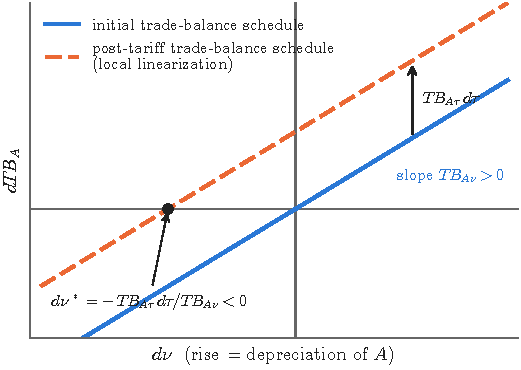
\includegraphics[width=0.65\textwidth]{fig1_bilateral.pdf}
\caption{Bilateral tariff and exchange-rate adjustment. At a fixed exchange rate, the tariff shifts the trade-balance schedule upward. When the Marshall--Lerner slope is positive, equilibrium is restored through an appreciation. Schematic.}
\label{fig:bilateral}
\end{figure}

\subsection{Multilateral adjustment}
\label{sec:representation}

Now consider $N$ countries, indexed by $\mathcal I=\{1,\dots,N\}$, and let $\mathcal I_{-A}=\mathcal I\setminus\{A\}$. Take $A$'s currency as numeraire. The $N-1$ bilateral rates $e_{Aj}$, $j\in\mathcal I_{-A}$, span all exchange-rate changes. Trade balances sum to zero (Walras' law), which leaves $N-1$ independent trade-balance conditions, indexed by $i\in\mathcal I_{-A}$:
\begin{equation*}
\TB_i\big(\{e_{Aj}\}_{j\in\mathcal I_{-A}},\{\tau_{jk}\}_{(j,k)\in\mathcal T}\big)=0,\qquad i\in\mathcal I_{-A},
\end{equation*}
where $\tau_{jk}$ is country $j$'s ad valorem tariff on imports from $k$ and $\mathcal T\equiv\{(j,k)\in\mathcal I\times\mathcal I:j\neq k\}$ is the set of all $N(N-1)$ ordered country pairs. Stack the bilateral rates as $\nu=(\nu_l)_{l\in\mathcal I_{-A}}$ with $\nu_l=\log e_{Al}$, in increasing order of $l$, and the tariffs as $\tau=(\tau_{jk})_{(j,k)\in\mathcal T}$, in lexicographic order of $(j,k)$. Linearizing,
\begin{equation}
J\,d\nu+G\,d\tau=0,\qquad J_{il}\equiv\frac{\partial\TB_i}{\partial\nu_l}\bigg|_{\tau},\qquad G_{i,(jk)}\equiv\frac{\partial\TB_i}{\partial\tau_{jk}}\bigg|_{\nu},
\label{eq:JG}
\end{equation}
for $i,l\in\mathcal I_{-A}$ and $(j,k)\in\mathcal T$, so $J\in\mathbb R^{(N-1)\times(N-1)}$ and $G\in\mathbb R^{(N-1)\times N(N-1)}$. Consider a tariff change along a fixed direction,
\begin{equation*}
d\tau=a\,ds,\qquad a\in\mathbb R^{N(N-1)},\quad\|a\|_2=1,
\end{equation*}
where the unit norm serves only to normalize the scalar $s$. Define $F\equiv Ga$, the marginal vector of trade-balance disturbances per unit increase in $s$, evaluated at unchanged exchange rates. Substituting into \cref{eq:JG},
\begin{equation*}
J\,\frac{d\nu}{ds}+Ga=0.
\end{equation*}
Provided $J$ is nonsingular, therefore,
\begin{equation}
\boxed{\;\frac{d\nu}{ds}=(-J)^{-1}F.\;}
\label{eq:response}
\end{equation}
\Cref{eq:response} separates the trade-balance effects of the tariff at unchanged exchange rates, $F$, which include expenditure switching, tariff revenue and income effects, from the exchange-rate movements required to restore external balance, $(-J)^{-1}$. In the bilateral case both are scalars, and \cref{eq:response} reduces to \cref{eq:bilat}. With $N\geq3$, however, the elements of $F$ need not have the same sign: a tariff imposed by $A$ on $B$ can improve a bystander $C$'s trade balance at unchanged exchange rates. The response of any bilateral exchange rate, including $\nu_C$, therefore depends on the full vector of tariff-induced trade-balance disturbances, not on its own element alone.

\subsection{A multilateral Marshall--Lerner condition}
\label{sec:mml}

\begin{definition}[Multilateral Marshall--Lerner condition, MML]
\label{def:mml}
Let $i,l\in\mathcal I_{-A}$. The adjustment mechanism satisfies MML if $J_{il}\geq0$ for every $l\neq i$, and $(-J)^{-1}$ exists with $(-J)^{-1}\geq0$ componentwise, that is, $[(-J)^{-1}]_{il}\geq0$ for all $i,l$. Equivalently, $-J$ is a nonsingular M-matrix.
\end{definition}

Under MML, writing $\vartheta_{ij}\equiv[(-J)^{-1}]_{ij}\geq0$,
\begin{equation}
\frac{d\nu_i}{ds}=\sum_{j\in\mathcal I_{-A}}\vartheta_{ij}F_j,\qquad i\in\mathcal I_{-A}.
\label{eq:signrule}
\end{equation}
Every disturbance enters every bilateral response with a nonnegative weight. Hence, componentwise, if $F\geq0$ then $d\nu/ds\geq0$, and if $F\leq0$ then $d\nu/ds\leq0$, where a positive $d\nu_i/ds$ is a depreciation of $A$ against $i$. This is the multilateral counterpart of the two-country result.

A primitive sufficient condition for MML is gross substitutability of trade balances, which is stated in terms of the full $N\times N$ Jacobian with respect to currency values. Let $\chi_l\equiv\log v_l$, $l\in\mathcal I$, be the log common-unit value of currency $l$. Since $e_{Aj}=v_j/v_A$,
\begin{equation*}
\nu_j=\chi_j-\chi_A,\qquad j\in\mathcal I_{-A}.
\end{equation*}
Define $\widetilde J_{il}\equiv\partial\TB_i/\partial\chi_l$ for $i,l\in\mathcal I$, at fixed tariffs. If each trade balance is homogeneous of degree one in currency values, Euler's identity gives $\sum_{l\in\mathcal I}\widetilde J_{il}=\TB_i=0$ at the balanced baseline, and Walras' law, $\sum_{i\in\mathcal I}\TB_i\equiv0$, gives $\sum_{i\in\mathcal I}\widetilde J_{il}=0$ for every $l\in\mathcal I$. Because $\chi_A$ is fixed by the normalization $v_A=1$, a change in $\nu_l$ is a change in $\chi_l$ alone, so the reduced Jacobian of \cref{eq:JG} is $J=(\widetilde J_{il})_{i,l\in\mathcal I_{-A}}$. Trade balances are gross substitutes if
\begin{equation*}
\widetilde J_{il}\geq0\qquad\text{for all }i,l\in\mathcal I,\ l\neq i,
\end{equation*}
that is, if an appreciation of currency $l$, a rise in $\chi_l$, weakly improves every other country's trade balance.

\begin{lemma}
\label{lem:gs}
If each trade balance is homogeneous of degree one in currency values, $\widetilde J_{il}\geq0$ for all $i,l\in\mathcal I$ with $l\neq i$, the reduced matrix $J=(\widetilde J_{il})_{i,l\in\mathcal I_{-A}}$ is irreducible, and $\widetilde J_{iA}>0$ for at least one $i\in\mathcal I_{-A}$, then MML holds.
\end{lemma}

\Cref{lem:gs} is the trade-balance analogue of the gross-substitutes stability results of \citet{hicks1939}, \citet{mosak1944}, \citet{metzler1945} and \citet{arrow1959}. MML ensures that multilateral adjustment is well behaved, and a disturbance vector of one sign produces exchange-rate responses of the same sign. When $F$ contains both positive and negative elements, however, MML alone does not determine the sign of an individual bilateral exchange-rate response. Positive own-exchange-rate trade-balance slopes are therefore not sufficient to sign bilateral responses in a multilateral setting.

\subsection{Symmetric trading partners}
\label{sec:decomposition}

\Cref{eq:response} holds at any balanced baseline. When the tariffing country's partners are symmetric, it can be solved using two eigenspace-specific eigenvalues of $-J$ and two of $G^{(A)}$.

Restrict attention to tariff changes imposed by $A$, $t=(t_j)_{j\in\mathcal I_{-A}}$ with $t_j\equiv d\tau_{Aj}$, and let $G^{(A)}\in\mathbb R^{(N-1)\times(N-1)}$ be the corresponding restriction of the tariff-incidence matrix,
\begin{equation*}
G^{(A)}_{ij}\equiv\frac{\partial\TB_i}{\partial\tau_{Aj}}\bigg|_{\nu},\qquad i,j\in\mathcal I_{-A},
\end{equation*}
so that $J\,d\nu+G^{(A)}t=0$. Assume that the primitives and the balanced baseline allocation are invariant to every relabeling of $A$'s $N-1$ partners. This implies that, for every $(N-1)\times(N-1)$ partner-permutation matrix $P$,
\begin{equation*}
PJP'=J\qquad\text{and}\qquad PG^{(A)}P'=G^{(A)}.
\end{equation*}
A free-trade or common-external-tariff baseline is an example only when the partner primitives are also symmetric. We then call $A$'s partners symmetric. With $\bone$ the $(N-1)$-vector of ones, decompose
\begin{equation}
t=\bar t\,\bone+\widetilde t,\qquad \bar t=\tfrac{1}{N-1}\bone't,\qquad \bone'\widetilde t=0.
\label{eq:tsplit}
\end{equation}
We call $\bar t$ \emph{average protection} and $\widetilde t$ \emph{relative treatment}. Any permutation-invariant matrix has the form $aI+b\bone\bone'$, so the one-dimensional common subspace $\operatorname{span}\{\bone\}$ and the $(N-2)$-dimensional deviation subspace $\{v:\bone'v=0\}$ are eigenspaces of both $G^{(A)}$ and $-J$:
\begin{equation*}
G^{(A)}\bone=g_S\bone,\quad G^{(A)}v=g_Dv;\qquad (-J)\bone=j_S\bone,\quad (-J)v=j_Dv\qquad(\bone'v=0).
\end{equation*}
The eigenvalues $j_D$ and $g_D$ each have multiplicity $N-2$.

We measure $A$'s effective exchange rate by its nominal effective exchange rate (NEER) with baseline bilateral trade weights. With $f_{ij}$ the border value of country $i$'s imports from $j$,
\begin{gather*}
w_{Aj}\equiv\frac{f_{Aj}+f_{jA}}{\sum_{k\neq A}(f_{Ak}+f_{kA})},\qquad \sum_{j\neq A}w_{Aj}=1,\\
E_A\equiv\prod_{j\neq A}e_{Aj}^{w_{Aj}},\qquad
d\nu^E_A\equiv d\log E_A=\sum_{j\neq A}w_{Aj}\,d\nu_j,
\end{gather*}
holding the baseline weights fixed for the local comparative static. This is the effective exchange rate throughout the paper. Under partner symmetry the bilateral trade weights are equal, $w_{Aj}=1/(N-1)$, so in this section the NEER reduces to the simple average of the bilateral log exchange rates, $d\nu^E_A=\frac{1}{N-1}\sum_{j\neq A}d\nu_j$. For partners $j,k\in\mathcal I_{-A}$ the cross rate is $e_{jk}=e_{Ak}/e_{Aj}$, units of $j$'s currency per unit of $k$'s.

\begin{proposition}[Average protection and relative treatment]
\label{prop:decomposition}
Let partners be symmetric, $N\geq3$, and $j_S,j_D\neq0$, so that $J$ is nonsingular. For any tariff vector $t$,
\begin{equation}
d\nu=\lambda_{\mathrm{avg}}\,\bar t\,\bone+\lambda_{\mathrm{rel}}\,\widetilde t,\qquad \lambda_{\mathrm{avg}}=\frac{g_S}{j_S},\quad \lambda_{\mathrm{rel}}=\frac{g_D}{j_D}.
\label{eq:decomp}
\end{equation}
Hence
\begin{equation}
d\nu^E_A=\lambda_{\mathrm{avg}}\bar t,\qquad d\nu_j-d\nu^E_A=\lambda_{\mathrm{rel}}\widetilde t_j,\qquad d\log e_{jk}=d\nu_k-d\nu_j=\lambda_{\mathrm{rel}}(t_k-t_j).
\label{eq:decompparts}
\end{equation}
Moreover, under the permutation-symmetry assumptions above, MML is equivalent to $j_S>0$ and $j_D\geq j_S$.
\end{proposition}

Average protection shifts all of $A$'s bilateral log exchange rates by the same amount, so under symmetry it determines the NEER. Relative treatment has zero mean, leaves the NEER unchanged, and moves bilateral rates around the common component; it also determines the movements in cross rates among partners. The two components lie in complementary subspaces, $\mathbb R^{N-1}=\operatorname{span}\{\bone\}\oplus\{v:\bone'v=0\}$, and each is scaled by its own coefficient. With $N=3$ these subspaces span a plane, which \cref{fig:geometry} uses to illustrate the decomposition.

\Cref{prop:decomposition} thus reduces the exchange-rate response to any tariff vector to two coefficients: $\lambda_{\mathrm{avg}}$, through which average protection moves the common component of $A$'s bilateral rates and hence its effective exchange rate, and $\lambda_{\mathrm{rel}}$, through which relative treatment moves individual bilateral rates around that component and the cross rates among partners. The decomposition follows from partner symmetry alone and does not rely on the nested-CES structure or any other particular demand system. What remains undetermined are the signs and magnitudes of $\lambda_{\mathrm{avg}}$ and $\lambda_{\mathrm{rel}}$, and hence the relative strength of the two components. \Cref{sec:nestedces} introduces a nested-CES model in which these coefficients depend on substitution between domestic and foreign goods and on substitution across foreign suppliers.

\section{The Nested-CES Model}
\label{sec:nestedces}

We now give economic content to these two components in a nested-CES trade model.

\subsection{Production, preferences and equilibrium}
\label{sec:model}

Each country $i\in\{1,\dots,N\}$ is endowed with $L_i$ units of labor, its size, which is mobile across sectors. It produces a country-specific tradable and a non-tradable with labor only, $Y_{Ti}=A_{Ti}L_{Ti}$ and $Y_{Ni}=A_{Ni}L_{Ni}$, with $L_{Ti}+L_{Ni}=L_i$. Normalizing each tradable's producer price to one in its own currency, $w_i=A_{Ti}$ and $P_{Ni}=A_{Ti}/A_{Ni}$. Relative international producer prices therefore move only through exchange rates, and \textbf{the bilateral exchange rate equals the bilateral terms of trade and the relative wage in a common currency.}

Preferences are
\begin{equation}
C_i=C_{Ti}^{\alpha_T}C_{Ni}^{1-\alpha_T},\quad
C_{Ti}=\Big[\alpha_D^{1/\eta}C_{Tii}^{\frac{\eta-1}{\eta}}+(1-\alpha_D)^{1/\eta}M_i^{\frac{\eta-1}{\eta}}\Big]^{\frac{\eta}{\eta-1}},\quad
M_i=\Big[\textstyle\sum_{j\neq i}\beta_{ij}^{1/\rho}C_{Tji}^{\frac{\rho-1}{\rho}}\Big]^{\frac{\rho}{\rho-1}}.
\label{eq:prefs}
\end{equation}
Here $\eta$ governs substitution between domestic tradables and the import composite, and $\rho$ substitution across foreign origins; the latter is inactive when $N=2$. Country $i$ levies $\tau_{ij}$ on imports from $j$, so the consumer price is $p_{ij}=(1+\tau_{ij})e_{ij}$, and the import and tradable price indices are $P_{Mi}=[\sum_{j\neq i}\beta_{ij}p_{ij}^{1-\rho}]^{1/(1-\rho)}$ and $P_{Ti}=[\alpha_D+(1-\alpha_D)P_{Mi}^{1-\eta}]^{1/(1-\eta)}$. Tariff revenue is rebated lump-sum, so income is
\begin{equation}
I_i=\frac{w_iL_i}{1-\sum_{j\neq i}\frac{\tau_{ij}}{1+\tau_{ij}}s_{ij}},
\label{eq:income}
\end{equation}
with $s_{ij}$ the realized tariff-inclusive expenditure share of income on $j$'s good. Trade balances are measured at border prices,
\begin{equation}
\TB_i=\sum_{k\neq i}f_{ki}-\sum_{j\neq i}f_{ij},\qquad f_{ij}=\frac{s_{ij}\tilde I_i}{1+\tau_{ij}},
\label{eq:tb}
\end{equation}
with $\tilde I_i=e_{Ai}I_i$ income in $A$'s currency. Under the normalization $v_A=1$ of \cref{sec:bilateral}, values in $A$'s currency equal values in the common unit of account, so \cref{eq:tb} is the trade-balance measure of \cref{sec:framework}: flows at border prices, with tariff revenue a domestic transfer. The NEER is the one defined in \cref{sec:decomposition}, written here for any country $i$: $E_i=\prod_{j\neq i}e_{ij}^{w_{ij}}$ with baseline trade weights $w_{ij}=(f_{ij}+f_{ji})/\sum_{k\neq i}(f_{ik}+f_{ki})$; throughout, ``effective exchange rate'' refers to this trade-weighted NEER. The real exchange rate is $q_{ij}=e_{ij}P_j/P_i$, with $P_i$ the consumer price index.

The \textbf{symmetric benchmark} is free trade with $\beta_{ij}=1/(N-1)$, common parameters, and equal endowments and productivities. It retains home bias $\alpha_D$. Write $m\equiv\alpha_T(1-\alpha_D)$ for the import share of income.

\subsection{The two-country case}
\label{sec:twocountry}

With one foreign supplier, linearizing gives $d\TB_A=mM_2\,d\nu_B+m\rho_D\,d\tau$, so
\begin{equation}
\begin{gathered}
\frac{d\log e_{AB}}{d\tau}\bigg|_{\tau=0}=-\frac{\rho_D}{M_2},\\
\rho_D\equiv\underbrace{\alpha_D\eta}_{\text{domestic substitution}}+\underbrace{(1-\alpha_D)(1-\alpha_T)}_{\text{rebate / non-tradables}},\qquad
M_2\equiv1+2\alpha_D(\eta-1)=\varepsilon_X+\varepsilon_M-1.
\end{gathered}
\label{eq:twocountry}
\end{equation}
$\rho_D$ is the \textbf{domestic diversion margin}. It measures how strongly a tariff pulls expenditure toward the domestic economy, through substitution toward the domestic tradable and through the rebate's income effect on non-tradables. An exchange-rate movement generates no revenue, so it has no rebate term. This is why $\rho_D\neq M_2$.

\subsection{The \texorpdfstring{$N$}{N}-country case}
\label{sec:theorem}

We now evaluate the eigenvalues of \cref{sec:decomposition} in this model.

\begin{theorem}[Exchange-rate responses in the symmetric nested-CES model]
\label{thm:main}
At the symmetric benchmark define
\begin{equation}
M_N\equiv\frac{1}{N-1}\Big[\,1+\underbrace{N\alpha_D(\eta-1)}_{\text{domestic--import adjustment}}+\underbrace{(N-2)\rho}_{\text{foreign-origin adjustment}}\Big].
\label{eq:MN}
\end{equation}
The eigenvalues of \cref{prop:decomposition} are (\cref{lem:jacobian} and \cref{eq:geigen})
\begin{equation}
g_S=-\frac{m\rho_D}{N-1},\qquad g_D=-\frac{m\rho}{N-1},\qquad j_S=\frac{mM_N}{N-1},\qquad j_D=Nj_S.
\label{eq:eigenvalues}
\end{equation}
MML holds if and only if $M_N>0$, and $\eta\geq1$ suffices. When it holds,
\begin{equation}
\lambda_{\mathrm{avg}}=-\frac{\rho_D}{M_N},\qquad \lambda_{\mathrm{rel}}=-\frac{\rho}{NM_N},\qquad d\nu_j=\lambda_{\mathrm{avg}}\bar t+\lambda_{\mathrm{rel}}\widetilde t_j.
\label{eq:lambdas}
\end{equation}
\end{theorem}

$M_N$ measures how sensitive $A$'s trade balance with the rest of the world is to its effective exchange rate: $d\TB_A=mM_N\,d\nu^E_A$, with the equal weights of the symmetric benchmark. When $N>2$ it includes $\rho$, because foreign buyers can substitute between $A$'s goods and other foreign goods. For $N=2$ it reduces to $M_2$. Average protection works as in the two-country case. Relative treatment is zero-sum, so to first order it leaves revenue, income and the tradable/non-tradable split unchanged, and its disturbance is governed by $\rho$ alone.

The factor $1/N$ in $\lambda_{\mathrm{rel}}$ is central. A common exchange-rate move shifts only partners' trade with $A$. A relative move also shifts partners' trade with \emph{each other}. At the symmetric benchmark $A$ accounts for a share $1/N$ of the trade on which relative movements act, so $j_D=Nj_S$. \textbf{Relative exchange-rate adjustment is $N$ times as effective as common adjustment}, and a given relative disturbance requires only $1/N$ as much exchange-rate movement.

\subsection{A unilateral tariff}
\label{sec:unilateral}

\begin{figure}[t]
\centering
\begin{subfigure}[t]{0.45\textwidth}\centering
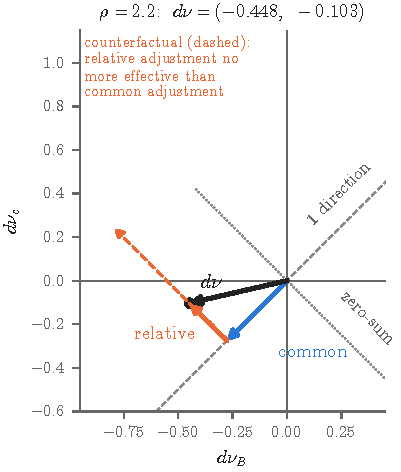
\includegraphics[width=\textwidth]{fig2a_geometry.pdf}
\caption{$\rho=2.2$: $\rho_D<\rho<3\rho_D$}
\label{fig:geometry-a}
\end{subfigure}\hfill
\begin{subfigure}[t]{0.45\textwidth}\centering
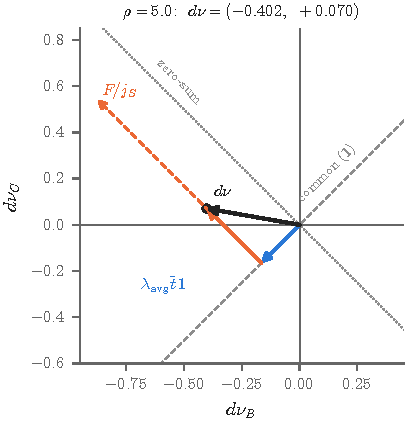
\includegraphics[width=\textwidth]{fig2b_geometry.pdf}
\caption{$\rho=5$: $\rho>3\rho_D$}
\label{fig:geometry-b}
\end{subfigure}
\caption{Average protection and relative treatment, $N=3$. A unilateral tariff on $B$, $t=(1,0)$, moves exchange rates through a common component (blue) and a relative component (solid orange); the black arrow is the equilibrium response $d\nu$, and the dashed arrow $F/j_S$ is the response if relative adjustment were no more effective than common adjustment. In (a), $C$'s trade balance improves at unchanged exchange rates, yet $A$ still appreciates against $C$. In (b), $A$ depreciates against $C$. The NEER appreciates in both. \textit{Notes:} $\alpha_D=0.7$, $\alpha_T=0.6$, $\eta=1.5$, so $\rho_D=1.17$ and $3\rho_D=3.51$.}
\label{fig:geometry}
\end{figure}

Let $A$ raise its tariff on $B$ alone, $t=d\tau\,e_B$. Then $\bar t=d\tau/(N-1)$, $\widetilde t_B=\frac{N-2}{N-1}d\tau$ and $\widetilde t_C=-\frac{d\tau}{N-1}$ for every bystander $C$.

\begin{proposition}[Unilateral tariff]
\label{prop:unilateral}
At the symmetric benchmark under MML,
\begin{equation}
\frac{d\nu^E_A}{d\tau}=-\frac{\rho_D}{(N-1)M_N}<0,\qquad
\frac{d\nu_B}{d\tau}=-\frac{N\rho_D+(N-2)\rho}{N(N-1)M_N}<0,\qquad
\frac{d\nu_C}{d\tau}=\frac{\rho-N\rho_D}{N(N-1)M_N}.
\label{eq:unilateral}
\end{equation}
\begin{enumerate}[label=(\roman*)]
\item $A$'s NEER appreciates for every $N$ and $\rho$.
\item $A$ appreciates against the target.
\item $A$ \textbf{depreciates against each untariffed bystander if and only if $\rho>N\rho_D$.}
\item The same threshold applies when $A$ tariffs any $k\leq N-2$ partners. More generally, $A$ depreciates against a partner $j$ facing a below-average tariff increase if and only if $t_j/\bar t<1-N\rho_D/\rho$, which requires $\rho>N\rho_D$.
\end{enumerate}
\end{proposition}

Against the target, average protection and relative treatment reinforce each other. Against a bystander they pull apart. Average protection shifts expenditure toward the domestic economy (appreciation), while the bystander's favorable relative treatment redirects expenditure toward it (depreciation).

\begin{corollary}[Why a single elasticity cannot deliver reversal]
\label{cor:single}
With home bias $\alpha_D\geq1/N$,
\begin{equation}
N\rho_D-\eta=\eta(N\alpha_D-1)+N(1-\alpha_D)(1-\alpha_T)\geq0,
\label{eq:single}
\end{equation}
so $\rho>\eta$ is \textbf{necessary} for a bystander depreciation. In any specification with a single elasticity across all tradable varieties ($\rho=\eta=\sigma$), $A$ appreciates against every bystander at every $\sigma$. At $\alpha_D=1/N$ the response is $-(1-\alpha_T)/(N\sigma)$, which approaches zero from below but never crosses it.
\end{corollary}

This explains why the natural first extension of the two-country model, a third country under a single CES elasticity, has not surfaced the reversal. The reversal requires that cross-origin substitution exceed home--import substitution, an ordering supported by the macro--micro elasticity evidence \citep{feenstra2018,li2022}. At US-like parameters ($\alpha_D=0.8$, $\alpha_T=0.4$, $\eta=1.5$, so $\rho_D=1.32$), $N\rho_D=3.96$ for $N=3$.

\paragraph{Disturbance versus equilibrium.} At unchanged exchange rates the bystander's trade balance improves if and only if $\rho>\rho_D$:
\begin{equation}
F_C=\frac{m(\rho-\rho_D)}{(N-1)^2}.
\label{eq:FC}
\end{equation}
The equilibrium bystander depreciation requires the stronger condition $\rho>N\rho_D$. The gap is the $1/N$ effectiveness of relative adjustment. For $\rho_D<\rho<N\rho_D$, $C$ gains at the old exchange rates yet ends up with a weaker currency against $A$ (\cref{fig:geometry-a}). \Cref{fig:unilateral} plots the three responses against $\rho$.

\begin{figure}[t]
\centering
\begin{subfigure}[t]{0.45\textwidth}\centering
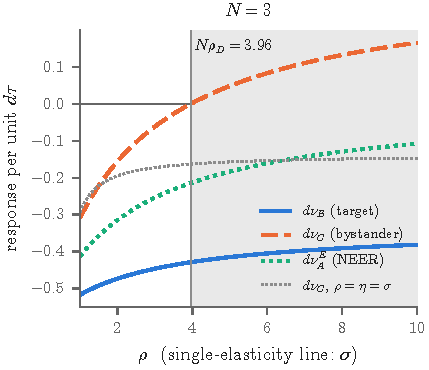
\includegraphics[width=\textwidth]{fig3a_unilateral.pdf}
\caption{$N=3$}
\end{subfigure}\hfill
\begin{subfigure}[t]{0.45\textwidth}\centering
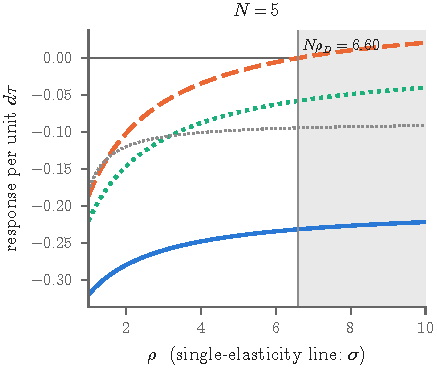
\includegraphics[width=\textwidth]{fig3b_unilateral.pdf}
\caption{$N=5$}
\end{subfigure}
\caption{Bilateral and effective responses to a unilateral tariff, per unit $d\tau$, US-like parameters ($\alpha_D=0.8$, $\alpha_T=0.4$, $\eta=1.5$). $d\nu_B$ and $d\nu^E_A$ are negative for every $\rho$; $d\nu_C$ crosses zero at $N\rho_D$ ($3.96$ for $N=3$, $6.60$ for $N=5$), and the shaded region is $\rho>N\rho_D$. The grey dotted line is the single-elasticity case $\rho=\eta=\sigma$, plotting $d\nu_C$ against $\sigma$; it never crosses zero (\cref{cor:single}). Closed forms of \cref{prop:unilateral}, verified against the linear solver.}
\label{fig:unilateral}
\end{figure}

\subsection{The three-country representation}
\label{sec:composite}

The $N$-country results can be read through a three-country economy, which we use as the workhorse for intuition. When the $N-2$ bystanders are symmetric and the tariff shock preserves that symmetry, no relative-price movement within the bystander bloc is activated. The bloc then has a single active direction, and the tariff experiment reduces exactly to three regions: $A$, $B$ and a composite bystander $C$. We now show that this composite is itself a nested-CES country, and we identify its parameters.

\begin{proposition}[Exact three-country reduction]
\label{prop:composite}
At the symmetric benchmark, consider any tariff change among $A$, $B$ and the bystanders that is common across bystanders: tariffs by $A$ or $B$ on all bystanders, by all bystanders on $A$ or $B$, or between $A$ and $B$. To first order, the responses of $\nu_B$, of every bystander rate $\nu_C$ and of $A$'s NEER coincide with those of a three-country nested-CES economy $\{A,B,C\}$ in which:
\begin{itemize}
\item $C$ has income $y_C=N-2$;
\item $A$ and $B$ place import weight $\frac{N-2}{N-1}$ on $C$ and $\frac{1}{N-1}$ on each other;
\item $C$ places import weight $\tfrac12$ on each of $A$ and $B$, with cross-origin elasticity $\rho$;
\item $C$'s home share of tradables is $h_C=\alpha_D+(1-\alpha_D)\frac{N-3}{N-1}$, equivalently $(N-1)h_C=N-3+2\alpha_D$;
\item $C$'s home--import elasticity is
\begin{equation}
\boxed{\;\eta_C=\frac{(N-3)\rho+2\alpha_D\,\eta}{N-3+2\alpha_D}.\;}
\label{eq:etaC}
\end{equation}
\end{itemize}
\end{proposition}

\begin{proof}[Proof sketch]
All bystander goods have the same price change, so CES aggregation of $A$'s and $B$'s demand over bystander goods is exact. Trade within the bloc cancels from the bloc's trade balance; what remains is the bloc's demand for $A$'s and $B$'s goods. Measure prices in bystander currency, so bloc goods have $dp=0$, and write $S=dp_A+dp_B$ and $D=dp_A-dp_B$. A bystander's import price index moves by $S/(N-1)$, since $A$ and $B$ are 2 of its $N-1$ import origins. Hence
\begin{equation*}
d\log s_{cA}=(1-\rho)\tfrac{D}{2}+\Big[(1-\rho)\tfrac{N-3}{2(N-1)}+(1-\eta)\tfrac{\alpha_D}{N-1}\Big]S.
\end{equation*}
In the composite the import index moves by $S/2$, so $d\log s_{CA}=(1-\rho)\frac D2+(1-\eta_C)h_C\frac S2$. The $D$ terms coincide. Matching the $S$ terms gives $(1-\eta_C)(N-1)h_C=(1-\rho)(N-3)+2\alpha_D(1-\eta)$, which is \cref{eq:etaC}. The full proof is in \cref{app:proofs}.
\end{proof}

The reduction is first-order. At finite tariffs a CES with constant $\eta_C$ does not replicate the bloc. The shocks it covers include the retaliation and trade-war experiments of \cref{sec:tradewars}.

\paragraph{Interpretation.} The composite bystander differs from an ordinary large country in one respect. Most of each bystander's trade is with \emph{other bystanders}, whose goods sit in the same $\rho$-nest as $A$'s and $B$'s. Once collapsed, this internal trade becomes the composite's ``home'' trade, and it is substitutable at a blend of $\rho$ and $\eta$. When $\rho>\eta$, $\eta_C$ rises toward $\rho$ as $N$ grows. The bystander bloc becomes inward-looking ($h_C\to1$) and highly substitutable.

\paragraph{The reduced system.} In the composite economy the $2\times2$ system for $(\nu_B,\nu_C)$ is, with $c=mM_N/(N-1)$,
\begin{equation}
-J=c\begin{pmatrix}N-1&-(N-2)\\-(N-2)&2(N-2)\end{pmatrix},\qquad \det(-J)=c^2N(N-2),
\label{eq:reducedJ}
\end{equation}
and
\begin{equation}
d\nu_C=\frac{F_B+(N-1)F_c}{cN},\qquad d\nu_B=\frac{2F_B+(N-2)F_c}{cN},
\label{eq:reducedsol}
\end{equation}
where $F_B$ is the target's disturbance and $F_c$ each bystander's ($F_C=(N-2)F_c$). Under a unilateral tariff, $F_B=-m[\rho_D+(N-2)\rho]/(N-1)^2<0$ and $F_c=m(\rho-\rho_D)/(N-1)^2$. \Cref{eq:reducedsol} recovers \cref{eq:unilateral} and gives the bystander response a two-force reading:
\begin{itemize}
\item \textbf{diversion}, $(N-1)F_c$: expenditure diverted toward bystanders improves their position and strengthens their currencies;
\item \textbf{redirection}, $F_B$: the target loses access to $A$'s market and its currency must fall. This makes the target's goods cheaper for bystanders and drags bystander currencies down with it.
\end{itemize}
$A$ depreciates against the bystander if and only if diversion outweighs redirection, $(N-1)(\rho-\rho_D)>\rho_D+(N-2)\rho$, which is $\rho>N\rho_D$. These are the ``trade diversion'' and ``trade redirection'' forces of earlier versions of this paper, now with exact weights.

\paragraph{Why $N$ raises the threshold, and why size alone does not.} One might expect that adding countries is equivalent to enlarging the bystander. It is not. Hold the composite's flows fixed at their $N$-country values but give it an ordinary home--import elasticity $\eta$ instead of $\eta_C$. The bystander threshold then \emph{falls} slightly with $N$, consistent with the general result (\cref{app:asym-primitives}) that a larger bystander lowers the threshold. The true threshold $N\rho_D$ rises steeply (\cref{tab:composite,fig:composite}). What drives the $N$-dependence is the bloc's internal, highly substitutable trade, which makes relative exchange-rate adjustment $N$ times as effective as common adjustment and dilutes $A$'s footprint to $1/N$.

\begin{table}[t]
\centering
\caption{$N$ versus bystander size}
\label{tab:composite}
\begin{tabular}{ccccc}
\toprule
 & & \multicolumn{2}{c}{Composite bystander threshold} & \\
\cmidrule(lr){3-4}
$N$ & $N\rho_D$ (true) & with $\eta_C$ \cref{eq:etaC} & with ordinary $\eta$ & $\eta_C$ at $\rho=4$ \\
\midrule
\tabinput{tables/tab1_composite.tex}
\bottomrule
\end{tabular}

\vspace{4pt}
\begin{minipage}{0.92\textwidth}\footnotesize
\textit{Notes:} US-like parameters ($\alpha_D=0.8$, $\alpha_T=0.4$, $\eta=1.5$). Thresholds are the values of $\rho$ at which the bystander response to a unilateral tariff changes sign in the composite economy of \cref{prop:composite}, computed with the linear system of \cref{app:linear}. The ``ordinary $\eta$'' column keeps the composite's flows but replaces $\eta_C$ by $\eta$.
\end{minipage}
\end{table}

\begin{figure}[t]
\centering
\begin{subfigure}[t]{0.45\textwidth}\centering
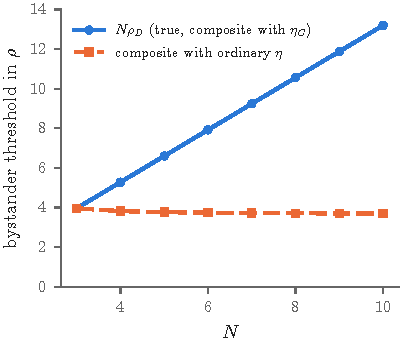
\includegraphics[width=\textwidth]{fig4a_composite_threshold.pdf}
\caption{Bystander threshold}
\end{subfigure}\hfill
\begin{subfigure}[t]{0.45\textwidth}\centering
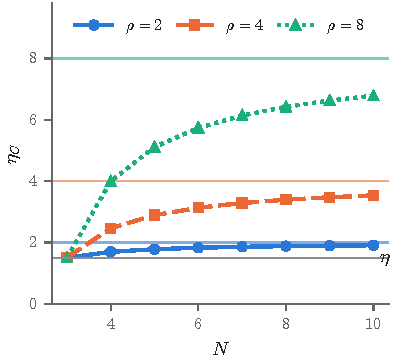
\includegraphics[width=\textwidth]{fig4b_eta_C.pdf}
\caption{Effective elasticity $\eta_C$}
\end{subfigure}
\caption{The composite bystander, US-like parameters. (a) The true threshold $N\rho_D$ for $N=3,\dots,10$, which the composite with $\eta_C$ reproduces exactly, and the threshold of the ``ordinary-$\eta$'' composite, which is nearly flat and slightly declining. (b) $\eta_C$ from \cref{eq:etaC} against $N$ for $\rho\in\{2,4,8\}$, converging toward $\rho$ (thin horizontal lines); the grey line is $\eta=1.5$.}
\label{fig:composite}
\end{figure}

\subsection{Real exchange rates}
\label{sec:real}

Real rates add a price-index wedge: the tariff raises $A$'s consumer prices directly. With $\bar t$ the average tariff and partners imposing no tariffs,
\begin{equation}
d\log q_{Aj}=\Big(1-\tfrac{mN}{N-1}\Big)d\nu_j-m\bar t,\qquad
dq^E_A=\Big[\Big(1-\tfrac{mN}{N-1}\Big)\lambda_{\mathrm{avg}}-m\Big]\bar t.
\label{eq:real}
\end{equation}

\begin{proposition}[Real exchange rates]
\label{prop:real}
Consider a unilateral tariff at the symmetric benchmark.
\begin{enumerate}[label=(\roman*)]
\item If $m<1/N$ and MML holds at the relevant $\rho$, the real bilateral threshold exceeds the nominal one:
\begin{equation*}
\rho^*_q(N)=\frac{[(N-1)-mN]N\rho_D+mN[N\alpha_D(\eta-1)+1]}{(N-1)(1-mN)}>N\rho_D.
\end{equation*}
\item If $m<(N-1)/N$, the REER appreciates.
\end{enumerate}
\end{proposition}

At US-like parameters and $N=3$, $\rho^*_q=4.93$, against $3\rho_D=3.96$.

\section{Trade Wars and Preferential Tariffs}
\label{sec:tradewars}

We now allow trading partners to respond. Since the analysis is local, simultaneous tariff changes by several countries add up.

\subsection{Trade wars}
\label{sec:retaliation}

\begin{proposition}[Retaliation and trade wars]
\label{prop:retaliation}
At the symmetric benchmark with $N\geq3$ under MML, to first order:
\begin{enumerate}[label=(\roman*)]
\item Under bilateral retaliation ($A$ tariffs $B$ and $B$ tariffs $A$ by $d\tau$), $d\nu_B=0$ and
\begin{equation}
\frac{d\nu_c}{d\tau}=\frac{\rho-\rho_D}{(N-1)M_N},\qquad
\frac{d\nu^E_A}{d\tau}=\frac{N-2}{N-1}\cdot\frac{\rho-\rho_D}{(N-1)M_N}.
\label{eq:retaliation}
\end{equation}
Both belligerents depreciate against every bystander, and in effective terms, if and only if $\rho>\rho_D$. Cross rates among bystanders are unchanged.
\item Under a multilateral trade war ($A$ tariffs every partner, and every partner retaliates against $A$), $d\nu_j=d\nu^E_A=\frac{(N-2)(\rho-\rho_D)}{(N-1)M_N}\,d\tau$ for all $j$, so $A$ depreciates against every partner if and only if $\rho>\rho_D$.
\end{enumerate}
\end{proposition}

$B$'s retaliation adds a second relative-treatment effect in the bystander's favor, which offsets the $1/N$ dilution. The bystander threshold therefore falls from $N\rho_D$ under a unilateral tariff to $\rho_D$, the point at which the bystander's trade balance improves at unchanged exchange rates. At the US-like calibration, $\rho_D=1.32$, below the illustrative range $\rho\in[2,4]$ shaded in \cref{fig:configurations}. Estimates in \citet{broda2006} and \citet{feenstra2018} place median cross-foreign elasticities around 3--4. For values in this range the model predicts that retaliation depreciates the tariffing country's currency against bystanders and in effective terms while leaving the belligerents' bilateral rate unchanged. The model can thus reproduce the pattern documented by \citet{ostry2025}, including the near-stability of the dollar against the renminbi in tit-for-tat episodes, with flexible prices, balanced trade and no financial channel.

The two experiments differ in where adjustment falls. Under bilateral retaliation the belligerents' rate is fixed and adjustment runs against bystanders. In a multilateral war there are no bystanders, and all of $A$'s rates move together.

\begin{figure}[t]
\centering
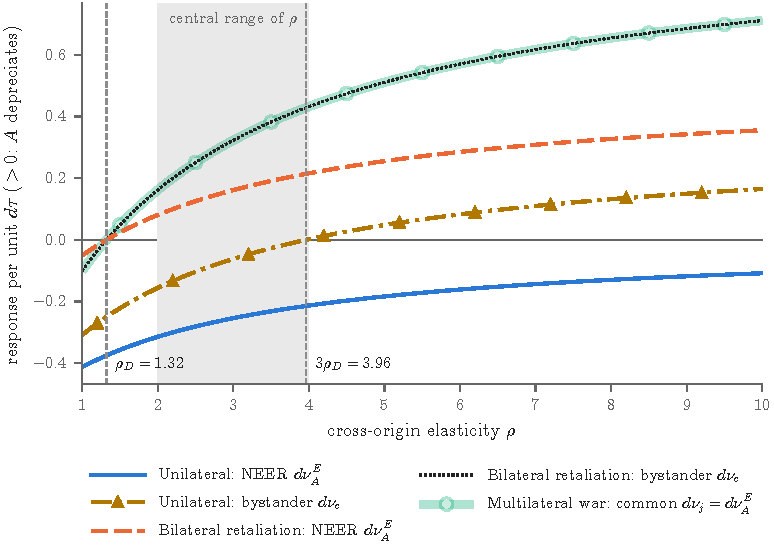
\includegraphics[width=0.8\textwidth]{fig5_configurations.pdf}
\caption{Exchange-rate responses across tariff configurations. Unilateral tariffs, bilateral retaliation, and a multilateral trade war for $N=3$. Retaliation lowers the bystander threshold from $3\rho_D$ to $\rho_D$. \textit{Notes:} US-like calibration; shading denotes $\rho\in[2,4]$.}
\label{fig:configurations}
\end{figure}

\subsection{Preferential tariffs and competing exporters}
\label{sec:pta}

In our model class the bystander's exchange rate is its terms of trade with $A$, $\ToT_{cA}=e_{Ac}$, so the response in \cref{eq:unilateral} is the third-country terms-of-trade effect of a discriminatory tariff, the central object of the preferential-trade-agreement literature since \citet{viner1950} and \citet{mundell1964}. In the canonical competing-exporter model, an importer $A$ that does not produce the good buys it from $B$ and $C$ under quasi-linear preferences. With $q_j$ exporter $j$'s price, $E_j$ its export supply and $M_A$ the importer's demand, a tariff on $B$ always improves $C$'s terms of trade,
\begin{equation*}
\frac{dq_C}{dt_B}=\frac{E'_B}{E'_B+E'_C-M'_A}>0.
\end{equation*}
In our model the bystander gains only if $\rho>N\rho_D$. The difference is that $A$ also produces a competing tradable: part of the demand diverted from $B$ goes to $A$'s own good, along with the rebate's income effect, so the third-country effect survives only when cross-origin substitution is strong relative to domestic diversion. \Cref{app:asym-tariff} shows that at a positive common external tariff the threshold rises, and that a discrete preferential cut requires a higher $\rho$ than the local threshold suggests.

\section{Asymmetry}
\label{sec:asymmetry}

Under partner symmetry the common and zero-sum subspaces are eigenspaces of the adjustment matrix (\cref{prop:decomposition}), so average protection moves the effective exchange rate and relative treatment moves bilateral rates around it. Asymmetry in country sizes, origin weights or home bias breaks this structure. This section asks which of the symmetric results survive. Two weighted averages of bilateral responses must be kept apart: the trade-weighted NEER of \cref{sec:decomposition}, with weights $w_{Aj}$ that combine $A$'s imports from and exports to $j$, and the aggregate terms of trade, which weight the same responses by $A$'s import shares $b_{Aj}$. The two coincide at the symmetric benchmark and differ away from it, and the second is the welfare-relevant object.

\subsection{The aggregate terms of trade and welfare}
\label{sec:welfare}

Let $b_{Aj}$ denote partner $j$'s share in $A$'s baseline import expenditure, so that $\sum_{j\neq A}b_{Aj}=1$, and let $R^B_j\equiv\partial\nu_j/\partial\tau_{AB}$ be the response of $A$'s bilateral rate against $j$ to a marginal tariff by $A$ on $B$; $R^B_j>0$ is a depreciation of $A$ against $j$. Define
\begin{equation}
R_{A|B}\equiv\sum_{j\neq A}b_{Aj}R^B_j.
\label{eq:RAB}
\end{equation}
Since each producer's price is fixed in its own currency, the log change in $A$'s import-weighted aggregate terms of trade is $-\sum_{j\neq A}b_{Aj}\,d\nu_j$, and a marginal tariff on $B$ improves it if and only if $R_{A|B}<0$.

The welfare result is stated at a balanced free-trade baseline of the model of \cref{sec:model} with interior shares, lump-sum rebate of tariff revenue, and exchange rates differentiable in tariffs, which holds whenever $J$ is nonsingular.

\begin{lemma}[First-order welfare]
\label{lem:welfare}
Under these assumptions, let $d\tau$ be any marginal tariff vector, imposed by $A$ or by other countries. To first order, the change in the welfare of $A$'s representative household, in units of $A$'s income, is
\begin{equation}
\frac{dU_A}{U_A'\,I_A}=-\,m_A\sum_{j\neq A}b_{Aj}\,d\nu_j,
\label{eq:welfare}
\end{equation}
where $m_A$ is $A$'s import share of income. A marginal tariff change therefore raises $A$'s own welfare to first order if and only if it improves $A$'s import-weighted aggregate terms of trade.
\end{lemma}

\noindent At free trade, the first-order tariff-revenue gain offsets the direct increase in import prices, leaving the welfare effect of the induced exchange-rate adjustment. The formal proof is in \cref{app:proofs}.

Because the first-order welfare effect is linear in the tariff vector, write, for tariffs imposed by $A$,
\begin{equation}
\frac{dU_A}{U_A'\,I_A}=\sum_{j\neq A}g_j\,d\tau_{Aj},\qquad g_j\equiv-m_A\,R_{A|j},
\label{eq:gradient}
\end{equation}
where $R_{A|j}$ is the response \cref{eq:RAB} to a tariff on $j$ alone. The component $g_j$ is the first-order welfare gain to $A$ from a marginal tariff on $j$, and a marginal uniform tariff, $d\tau_{Aj}=dt$ for all $j\neq A$, is worth $\sum_jg_j\,dt$.

\begin{proposition}[Uniform tariffs]
\label{prop:uniform}
Consider any balanced free-trade baseline at which MML and the assumptions of \cref{lem:welfare} hold; country sizes, origin shares, home biases and parameters may differ across countries. Let $A$ impose a marginal uniform tariff on all foreign partners, $d\tau_{Aj}=dt>0$ for all $j\neq A$, with all other tariffs unchanged. Then:
\begin{enumerate}[label=(\roman*)]
\item the tariff disturbs every partner's trade balance by
\begin{equation}
F_j=-f_{Aj}\,\rho_D^A\,dt,\qquad \rho_D^A\equiv\eta_Ah_A+(1-h_A)(1-\alpha_T^A)>0,
\label{eq:uniformF}
\end{equation}
where $h_A$ is $A$'s home share of tradable spending and $\eta_A$, $\alpha_T^A$ are $A$'s own parameters;
\item $A$'s currency appreciates weakly against every partner, $d\nu_j\leq0$, and strictly against every partner if $A$ imports from all of them or $J$ is irreducible;
\item $A$'s import-weighted aggregate terms of trade improve and $A$'s own welfare rises to first order: $\sum_{j\neq A}g_j>0$.
\end{enumerate}
\end{proposition}

\noindent A uniform tariff leaves relative import prices across foreign suppliers unchanged, so cross-origin substitution creates no differential incidence across partners, and the exchange-rate adjustment preserves the conventional aggregate result. The result is local, concerns $A$'s own welfare at a balanced free-trade baseline, and establishes nothing about finite tariffs, retaliation, global welfare, or a globally optimal tariff. It is a local, own-country counterpart of the classical terms-of-trade argument for a small tariff \citep{johnson1953,broda2008,costinot2015}; as in \citet{bagwell1999,bagwell2002}, nondiscrimination confines a country's tariffs to a single terms-of-trade channel. The proof is in \cref{app:proofs}.

A uniform tariff restricts the sum of the partner-specific welfare gradients, not every component separately; a tariff on one partner can therefore still lower $A$'s welfare. With $N=3$, $g_B+g_C>0$, so $g_B<0$ implies $g_C>0$.

\subsection{The aggregate terms-of-trade condition}
\label{sec:totcondition}

Separate the target from the remaining suppliers. Define
\begin{equation*}
\bar R^B_{-B}\equiv\frac{\sum_{j\neq A,B}b_{Aj}R^B_j}{1-b_{AB}},
\end{equation*}
the import-weighted average response of $A$'s rates against all bystanders, each bystander weighted by its share in $A$'s imports from suppliers other than $B$. Then $R_{A|B}=b_{AB}R^B_B+(1-b_{AB})\bar R^B_{-B}$: $A$'s exposure to the target, its import weight on $B$ times the move against $B$, plus its exposure to the bystanders.

\begin{definition}[Aggregate terms-of-trade condition]
\label{def:tot}
Unilateral tariffs by $A$ have the conventional aggregate terms-of-trade effect if, for every target $B$,
\begin{equation}
b_{AB}R^B_B+(1-b_{AB})\bar R^B_{-B}<0.
\label{eq:totcondition}
\end{equation}
\end{definition}

Suppose $A$ appreciates against the target, $R^B_B<0$, and depreciates on average against the bystanders, $\bar R^B_{-B}>0$. The condition then fails if and only if
\begin{equation}
\frac{\bar R^B_{-B}}{-R^B_B}>\frac{b_{AB}}{1-b_{AB}}.
\label{eq:totfail}
\end{equation}
The left side is the \emph{equilibrium incidence}: the average adverse move against bystanders per unit of favorable move against the target. The right side is \emph{relative import exposure}: $A$'s import expenditure on the target relative to its import expenditure on all other suppliers. Both are positive pure numbers. Given $R^B_B<0$, a bilateral reversal against at least one bystander is necessary but not sufficient for an aggregate reversal: the adverse moves must also be large enough and carry enough weight in $A$'s import basket.

In terms of \cref{eq:gradient}, the condition requires every partner-specific component $g_B$ to be positive, whereas \cref{prop:uniform} restricts only their sum. The condition has a three-country algebraic form for any configuration of bystanders, because $\bar R^B_{-B}$ is defined as their import-weighted average; this does not make a heterogeneous bloc a literal representative country (\cref{sec:heterogeneous}).

\subsection{Asymmetric partners in the three-country model}
\label{sec:threecountry}

Fix a balanced free-trade baseline of the three-country model, that is, the import-origin shares $b_{ij}$, the home shares $h_i$, the incomes $y_i$ and all parameters other than $\rho$, and let only $\rho$ vary. Write the local system as $A(\rho)R=F(\rho)$, with $A\equiv-J$ and $R=(R^B_B,R^B_C)'$. Since $\rho$ enters the linearized share responses (\cref{eq:linear}) only through the factor $(1-\rho)$, every entry of $A$ and $F$ is affine in $\rho$, and so is the adjugate of the $2\times2$ matrix $A$. Hence
\begin{equation}
R_{A|B}(\rho)=\frac{b'\adj(A(\rho))F(\rho)}{\det A(\rho)},\qquad
b'\adj(A(\rho))F(\rho)=q_2\rho^2+q_1\rho+q_0\equiv Q_{A|B}(\rho).
\label{eq:Q}
\end{equation}
Under MML $\det A(\rho)>0$, so at every $\rho$ at which MML holds at the fixed baseline, $R_{A|B}$ has the sign of $Q_{A|B}(\rho)$ and the aggregate condition is $Q_{A|B}(\rho)<0$. The bilateral bystander response has the same structure; with a common $\alpha_T$, its numerator has leading coefficient $\alpha_T^2\,b_{AB}b_{AC}b_{CA}b_{CB}(1-h_A)(1-h_C)y_Ay_C>0$ (\cref{app:asym-primitives}).

\begin{proposition}[Three cases]
\label{prop:threecases}
Fix a balanced free-trade baseline of the three-country model as above, and consider values $\rho>0$ at which MML holds at that baseline. The following three cases are those used in this paper; they are not an exhaustive classification of the signs of $(q_2,q_1,q_0)$.
\begin{enumerate}[label=(\alph*)]
\item Symmetric benchmark: $q_2=0$ and $Q_{A|B}(\rho)<0$ for all $\rho$. The aggregate condition always holds.
\item $q_2>0$ and $q_0<0$: $Q_{A|B}$ has exactly one positive root $\rho^*$. The condition holds for $\rho<\rho^*$ and fails for $\rho>\rho^*$.
\item $q_2<0$, $q_1>0$, $q_0<0$ and a positive discriminant: $Q_{A|B}$ has two positive roots $\rho_1<\rho_2$. The condition fails only for $\rho_1<\rho<\rho_2$.
\end{enumerate}
\end{proposition}

Case (b) is the economically central asymmetric case: the conventional aggregate effect holds at low cross-origin substitutability and is reversed above a single threshold. Case (c) requires richer network asymmetry and is reported as a robustness example. The three panels of \cref{fig:tot} are parameterized examples of the three cases (\cref{app:asym-tot}).

\begin{figure}[t]
\centering
\begin{subfigure}[t]{0.32\textwidth}\centering
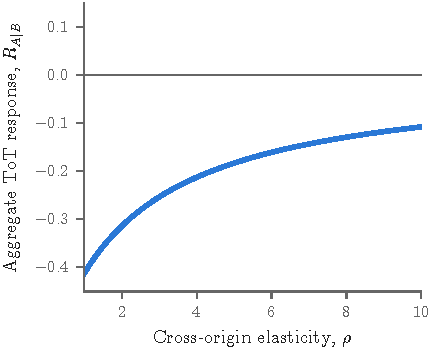
\includegraphics[width=\textwidth]{fig6a_aggregate_tot.pdf}
\caption{Symmetric benchmark}
\end{subfigure}\hfill
\begin{subfigure}[t]{0.32\textwidth}\centering
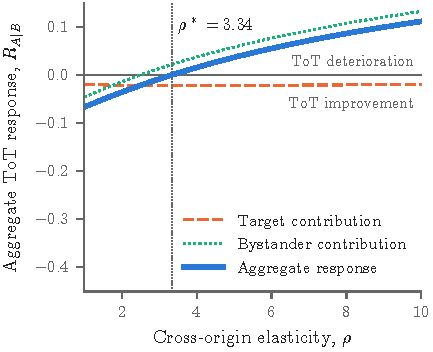
\includegraphics[width=\textwidth]{fig6b_aggregate_tot.pdf}
\caption{Small, low-weight target}
\end{subfigure}\hfill
\begin{subfigure}[t]{0.32\textwidth}\centering
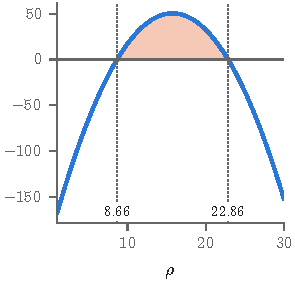
\includegraphics[width=\textwidth]{fig6c_aggregate_tot.pdf}
\caption{Asymmetric network}
\end{subfigure}
\caption{Aggregate terms-of-trade effects under asymmetry. Examples with no reversal, one threshold, and two thresholds. Shading denotes regions in which a marginal discriminatory tariff worsens the aggregate terms of trade.}
\label{fig:tot}
\end{figure}

Aggregate terms-of-trade reversal is more likely when the targeted partner is small relative to untariffed suppliers, when it has a low weight in $A$'s imports, and when foreign suppliers are sufficiently close substitutes. The appreciation against a small or lightly weighted target receives little weight in $A$'s import price index, the adverse movements against larger bystanders receive more, and strong cross-origin substitution redirects expenditure toward those bystanders. In the local model, at a balanced free-trade baseline satisfying MML, a discriminatory marginal tariff can therefore reduce $A$'s own welfare to first order, whereas by \cref{prop:uniform} a marginal uniform tariff at the same baseline raises it. \Cref{app:asym-tot} reports the numerical examples.

\subsection{Effective exchange rates and heterogeneous bystanders}
\label{sec:neer}
\label{sec:heterogeneous}

The NEER uses trade weights $w_{Aj}$, which include $A$'s exports to $j$, whereas the aggregate terms of trade use import weights $b_{Aj}$. Under asymmetry the two weighting schemes differ, so the NEER threshold can differ from the aggregate terms-of-trade threshold; when the target buys much more from $A$ than $A$ buys from it, the favorable move against the target counts for more in the NEER. \Cref{app:asym-tot} reports a numerical illustration.

For $N\geq4$, heterogeneous bystanders generally cannot be collapsed into the exact representative bystander of \cref{prop:composite}. The bloc's average response depends on its internal adjustment structure, including the block $J_{RR}$ of bystanders' responses to their own rates, their responses $J_{RB}$ to the rate against the target, and their disturbances $F_R$ (\cref{app:asym-primitives}), even though the identity $R_{A|B}=b_{AB}R^B_B+(1-b_{AB})\bar R^B_{-B}$ always holds. The three-country structure is therefore a diagnostic of sign mechanisms rather than a quantitative representation of a heterogeneous network.

\subsection{A stylized reading of the 2025 episode}
\label{sec:2025}

The 2025 exercise is neither a calibration nor a causal test. The model is static, has flexible prices, and is evaluated around balanced trade, while observed exchange rates are high-frequency asset prices affected by many contemporaneous shocks. We use the model only to classify the sign patterns associated with different tariff configurations. For each phase, we identify the tariff configuration, state the sign pattern associated with that configuration, compare it with the observed exchange-rate movements, and limit the inference to sign consistency.

Observed exchange-rate movements do not identify $\rho$, $\rho_D$, or the contribution of the trade mechanism. A movement is described as consistent with the model only when its sign matches the model's sign under the stated tariff configuration and parameter condition. \Cref{tab:phases} and \cref{fig:episode} report the data, with a positive number a depreciation of the dollar; the Federal Reserve's broad dollar index is the closest counterpart of the model's trade-weighted NEER, and the index excluding China isolates the bystanders.

\begin{table}[t]
\centering
\caption{Exchange-rate changes within the three phases of the 2025 episode (percent; positive = dollar depreciation)}
\label{tab:phases}
\small
\begin{tabular}{lcccccc}
\toprule
 & \multicolumn{2}{c}{Phase 1} & \multicolumn{2}{c}{Phase 2} & \multicolumn{2}{c}{Phase 3} \\
 & \multicolumn{2}{c}{Feb~1--Apr~2} & \multicolumn{2}{c}{Apr~3--May~12} & \multicolumn{2}{c}{Aug~7--Dec~31} \\
\cmidrule(lr){2-3}\cmidrule(lr){4-5}\cmidrule(lr){6-7}
 & Monthly & Daily & Monthly & Daily & Monthly & Daily \\
\midrule
\tabinput{tables/tab6_phases.tex}
\bottomrule
\end{tabular}

\vspace{4pt}
\begin{minipage}{0.95\textwidth}\footnotesize
\textit{Notes:} Monthly columns compare monthly averages (January with March, March with April, July with December); daily columns compare the last available observations at the phase boundaries (January~31 to April~2, April~2 to May~12, August~6 to December~31). VND daily entries (marked $^{a}$) use BIS end-of-month rates. Sources: Federal Reserve H.10 and BIS; see \cref{app:episode-data}.
\end{minipage}
\end{table}

\paragraph{Phase 1: China-focused escalation (February~1--April~2).} The United States raised tariffs on China, while China responded with narrower product-specific tariffs. The United States also imposed tariffs on Canada and Mexico, and Canada retaliated, so this phase is not a clean unilateral-tariff experiment. Approximating it as a tariff concentrated on China, \cref{prop:unilateral} associates the configuration with dollar appreciation against the target and, when $\rho>N\rho_D$, depreciation against untariffed bystanders. The dollar was approximately unchanged against the renminbi and weakened against the euro and the broad index excluding China. The bystander movements are consistent with the high-$\rho$ sign pattern, but the mixed tariff configuration and contemporaneous shocks prevent a sharper inference.

\begin{figure}[t]
\centering
\begin{subfigure}[t]{0.9\textwidth}\centering
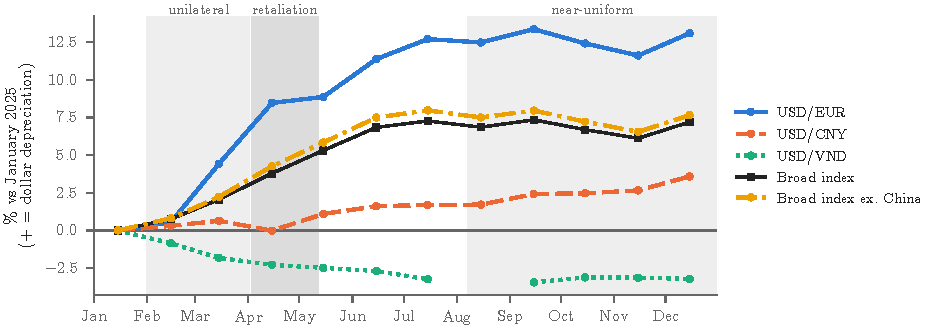
\includegraphics[width=\textwidth]{fig7a_fx2025.pdf}
\caption{Exchange rates, percent deviation from the January~2025 average (positive = dollar depreciation)}
\end{subfigure}

\vspace{6pt}
\begin{subfigure}[t]{0.9\textwidth}\centering
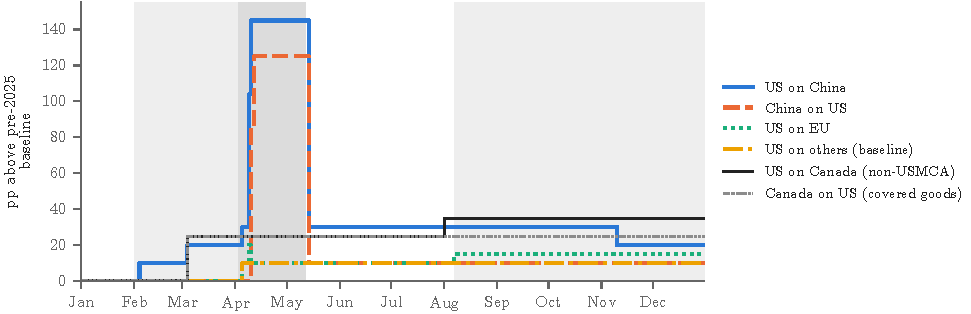
\includegraphics[width=\textwidth]{fig7b_tariffs2025.pdf}
\caption{Headline tariff increases above the pre-2025 baseline (percentage points)}
\end{subfigure}
\caption{Exchange rates and headline tariff increases during 2025. Shading denotes the three policy phases. Sources: Federal Reserve, BIS, Federal Register, Department of Finance Canada, and China's State Council Tariff Commission.}
\label{fig:episode}
\end{figure}

\paragraph{Phase 2: US--China retaliation (April~3--May~12).} The United States and China raised tariffs sharply against each other, while most other partners faced a common 10 percent US baseline tariff. The configuration is therefore closest to bilateral retaliation with an additional uniform component. \Cref{prop:retaliation} associates bilateral retaliation with a stable rate between the belligerents and, when $\rho>\rho_D$, depreciation against bystanders and in effective terms. During the phase, the dollar moved little against the renminbi but depreciated against the euro, the broad index excluding China, and the full broad index. This is the phase most closely aligned with the retaliation sign pattern. The comparison establishes sign consistency only; it does not identify the relevant elasticity or the contribution of the trade mechanism.

\paragraph{Phase 3: Near-uniform tariffs with residual retaliation (August~7--December~31).} US tariffs became more nearly uniform across partners, although higher rates and retaliation remained for some countries. The broader uniform component strengthens the average-protection channel, which pushes toward effective dollar appreciation, while the remaining discriminatory and retaliatory components can push in the opposite direction. The broad dollar index was approximately flat within the phase, with no clear effective appreciation. Over 2025 as a whole, the dollar depreciated substantially, by $7.2$ percent against the broad index and $7.6$ percent against the index excluding China between the January and December monthly averages, with most of that movement occurring before August. The static trade mechanism therefore does not account for the full effective depreciation. A quantitative assessment would require the complete tariff network, substitution elasticities, trade weights, retaliation, and a dynamic mechanism linking expected policy to asset prices.

The comparison across phases is more informative than any individual episode. A configuration dominated by bilateral retaliation is associated with stronger bystander and effective depreciation forces, while broader uniform protection strengthens the average-protection force. The observed movements in Phase~2 have the sign pattern associated with retaliation, whereas Phase~3 provides no corresponding broad appreciation as protection became more uniform. These comparisons illustrate the importance of the tariff configuration without identifying tariffs as the cause of the exchange-rate movements.

\FloatBarrier

\section{Conclusion}
\label{sec:conclusion}

In a two-country world, the bilateral exchange rate, the effective exchange rate and the terms of trade coincide, and a tariff appreciates the tariffing country's currency wherever Marshall--Lerner holds. In a multilateral world they separate. We have characterized what the real trade channel implies once they do.

The general response is the inverse of a multilateral adjustment matrix applied to a vector of tariff disturbances. A multilateral Marshall--Lerner condition makes adjustment well behaved without fixing the sign of any bilateral response. Under symmetry, average protection moves the effective rate and relative treatment moves bilateral rates around it. In a nested-CES model the conventional result survives exactly at the effective level under unilateral tariffs. It fails bilaterally against bystanders when cross-origin substitution exceeds $N$ times the domestic diversion margin, and against everyone under retaliation once it exceeds the domestic diversion margin itself. An exact three-country representation shows that the role of $N$ comes from the inward-looking, highly substitutable trade of the bystander bloc, not from its size. Under asymmetry, even the effective and welfare-relevant conclusions can fail: tariffing a small, lightly weighted partner whose goods are easily replaced can worsen the tariffing country's aggregate terms of trade.

The implications run both ways. Appreciation against a tariffed partner is not evidence of broad currency strength. A multilateral depreciation during a discriminatory or retaliatory tariff episode cannot be attributed to financial channels on the basis of the two-country prediction alone. Conversely, when tariffs are nearly uniform, the trade channel predicts effective appreciation, and observed weakness must come from elsewhere.

Natural next steps are to embed the decomposition in a quantitative multi-country model with input--output linkages and heterogeneous elasticities, and to add nominal rigidities, invoicing and a financial account. This would let the long-run real benchmark derived here interact with the short-run monetary and portfolio dynamics that dominate exchange rates at business-cycle frequencies.


\clearpage
\singlespacing
\bibliographystyle{aer}
\bibliography{refs}
\onehalfspacing

\appendix
\crefalias{section}{appendix}
\crefalias{subsection}{appendix}
\counterwithin{figure}{section}
\section{The Linearized System}
\label{app:linear}

This appendix derives the linear system \cref{eq:JG} of the nested-CES model of \cref{sec:model} and evaluates it at the symmetric benchmark.

\subsection{General linearization}

All derivatives are first-order and evaluated at a balanced free-trade baseline, $\tau_{ij}=0$ and $\TB_i=0$ for every $i\in\mathcal I$. Values are in the common unit of account of \cref{sec:bilateral}, with $v_A=1$. Write $\chi_l=\log v_l$ for $l\in\mathcal I$; then $\nu_j=\log e_{Aj}=\chi_j-\chi_A$, $\nu_A\equiv0$, and $d\log e_{ij}=d\nu_j-d\nu_i$.

The baseline is described by origin shares $b_{ij}$ within $i$'s import bundle ($b_{ii}=0$, $\sum_{j\neq i}b_{ij}=1$), home shares $h_i$ of $i$'s tradable spending, and incomes $y_i\equiv\tilde I_i$ in the common unit. The share of $i$'s income spent on $j$'s good is $s_{ij}=\alpha_T^i(1-h_i)b_{ij}$, and the border value of $i$'s imports from $j$ is $f_{ij}=s_{ij}y_i$; $\eta_i$, $\rho_i$ and $\alpha_T^i$ may differ by country. Log-differentiating the price indices of \cref{sec:model}, the demand system \cref{eq:prefs}, income \cref{eq:income} and the trade balance \cref{eq:tb} gives
\begin{equation}
\begin{aligned}
dp_{ij}&=d\nu_j-d\nu_i+d\tau_{ij},\qquad dp_{ii}=0,\\
d\log P_{Mi}&=\textstyle\sum_{j\neq i}b_{ij}\,dp_{ij},\qquad d\log P_{Ti}=(1-h_i)\,d\log P_{Mi},\\
d\log s_{ii}&=-(1-\eta_i)(1-h_i)\,d\log P_{Mi},\\
d\log s_{ij}&=(1-\rho_i)(dp_{ij}-d\log P_{Mi})+(1-\eta_i)h_i\,d\log P_{Mi},\\
d\log\tilde I_i&=d\nu_i+\textstyle\sum_{j\neq i}s_{ij}\,d\tau_{ij},\\
d\TB_i&=\textstyle\sum_{k\neq i}f_{ki}(d\log s_{ki}+d\log\tilde I_k-d\tau_{ki})-\sum_{j\neq i}f_{ij}(d\log s_{ij}+d\log\tilde I_i-d\tau_{ij}),
\end{aligned}
\label{eq:linear}
\end{equation}
where $dp_{ij}$ is the log change in $i$'s consumer price of $j$'s good in $i$'s currency. At free trade, only the direct revenue term survives in $d\log\tilde I_i$, and $d\log f_{ij}=d\log s_{ij}+d\log\tilde I_i-d\tau_{ij}$. Stacking the trade-balance equations gives the matrices $J$ and $G$ in \cref{eq:JG}.

\subsection{The symmetric benchmark}

At the symmetric benchmark the country subscripts on $\eta$, $\rho$ and $\alpha_T$ are dropped; $b_{ij}=1/(N-1)$, $h_i=\alpha_D$, $y_i=1$, and $f_{ij}=s_{ij}=m/(N-1)$ with $m=\alpha_T(1-\alpha_D)$.

\begin{lemma}[Jacobian at the symmetric baseline]
\label{lem:jacobian}
At the symmetric balanced baseline, $\widetilde J_{il}=mM_N/(N-1)$ for $i,l\in\mathcal I$ with $l\neq i$, and $\widetilde J_{ii}=-mM_N$. The reduced matrix $J=(\widetilde J_{il})_{i,l\in\mathcal I_{-A}}$ satisfies
\begin{equation}
-J=j_S\,(NI-\bone\bone'),\qquad j_S=\frac{mM_N}{N-1},\qquad j_D=Nj_S.
\label{eq:Jsym}
\end{equation}
\end{lemma}

\begin{proof}
Substituting the symmetric baseline into \cref{eq:linear} gives $\widetilde J_{il}=mM_N/(N-1)$ for $i\neq l$. Homogeneity and balanced trade imply zero row sums, giving $\widetilde J_{ii}=-mM_N$. Deleting the numeraire row and column yields \cref{eq:Jsym}. The corresponding tariff disturbance follows from \cref{eq:linear} at $d\nu=0$, giving \cref{eq:disturbance} and the eigenvalues in \cref{eq:geigen}. Detailed differentiation is reported in the online supplement.
\end{proof}

At $d\nu=0$, a change $t=(t_j)_{j\in\mathcal I_{-A}}$, $t_j=d\tau_{Aj}$, in $A$'s tariffs moves only $A$'s import prices and income, so among $A$'s partners only $i$'s exports to $A$ change:
\begin{equation}
d\TB_i\big|_{\nu}=f_{Ai}\big(d\log s_{Ai}+d\log\tilde I_A-t_i\big)=\frac{m}{N-1}\Big[-\rho_D\,\bar t-\rho\,(t_i-\bar t)\Big],
\label{eq:disturbance}
\end{equation}
using $d\log P_{MA}=\bar t$, $d\log s_{Ai}=(1-\rho)(t_i-\bar t)+(1-\eta)\alpha_D\bar t$, $d\log\tilde I_A=m\bar t$ and $1-(1-\eta)\alpha_D-m=\rho_D$. Equivalently, $G^{(A)}=\frac{m}{N-1}\big[-\rho I+\frac{\rho-\rho_D}{N-1}\bone\bone'\big]$, with eigenvalues
\begin{equation}
g_S=-\frac{m\rho_D}{N-1},\qquad g_D=-\frac{m\rho}{N-1},
\label{eq:geigen}
\end{equation}
on $\operatorname{span}\{\bone\}$ and on the zero-sum subspace.

\subsection{The two-country case}
\label{app:linear-twocountry}

At $N=2$ the margin $(1-\rho)$ is inactive, $dp_{AB}=d\log P_{MA}=d\nu_B+d\tau$ and $dp_{BA}=d\log P_{MB}=-d\nu_B$, so
\begin{equation*}
\begin{aligned}
d\log s_{AB}&=(1-\eta)\alpha_D(d\nu_B+d\tau),&\qquad d\log s_{BA}&=-(1-\eta)\alpha_D\,d\nu_B,\\
d\log\tilde I_A&=m\,d\tau,&\qquad d\log\tilde I_B&=d\nu_B.
\end{aligned}
\end{equation*}
Substituting into $\TB_A=f_{BA}-f_{AB}$,
\begin{equation*}
d\TB_A=m\Big[\big(1+2\alpha_D(\eta-1)\big)d\nu_B+\big(1-m+\alpha_D(\eta-1)\big)d\tau\Big]=mM_2\,d\nu_B+m\rho_D\,d\tau,
\end{equation*}
with $M_2=1+2\alpha_D(\eta-1)$ and $\rho_D=1-m+\alpha_D(\eta-1)=\alpha_D\eta+(1-\alpha_D)(1-\alpha_T)$. Setting $d\TB_A=0$ gives \cref{eq:twocountry}.

At the balanced free-trade baseline, the corresponding import and export elasticities satisfy $\varepsilon_X+\varepsilon_M-1=M_2$, so $M_2>0$ is the Marshall--Lerner condition used in \cref{sec:twocountry}.

\subsection{Unilateral tariffs}
\label{app:linear-unilateral}

Here $N\geq3$, the baseline is the symmetric benchmark, and $M_N>0$. For a unilateral tariff, $t=d\tau\,e_B$, and an individual bystander $c$, $\bar t=d\tau/(N-1)$, $\widetilde t_B=\frac{N-2}{N-1}d\tau$ and $\widetilde t_c=-\frac{d\tau}{N-1}$. By \cref{eq:lambdas},
\begin{equation*}
\begin{aligned}
d\nu_B&=\frac{\lambda_{\mathrm{avg}}+(N-2)\lambda_{\mathrm{rel}}}{N-1}\,d\tau=-\frac{N\rho_D+(N-2)\rho}{N(N-1)M_N}\,d\tau,\\
d\nu_c&=\frac{\lambda_{\mathrm{avg}}-\lambda_{\mathrm{rel}}}{N-1}\,d\tau=\frac{\rho-N\rho_D}{N(N-1)M_N}\,d\tau,\qquad
d\nu^E_A=\frac{\lambda_{\mathrm{avg}}}{N-1}\,d\tau=-\frac{\rho_D}{(N-1)M_N}\,d\tau,
\end{aligned}
\end{equation*}
which is \cref{eq:unilateral}; $d\nu_c>0$ if and only if $\rho>N\rho_D$. By \cref{eq:disturbance}, the target's and each bystander's disturbances per unit $d\tau$ are
\begin{equation*}
F_B=-\frac{m[\rho_D+(N-2)\rho]}{(N-1)^2}<0,\qquad F_c=\frac{m(\rho-\rho_D)}{(N-1)^2},
\end{equation*}
the second of which is \cref{eq:FC}. For a general tariff vector with $\bar t>0$, substituting $\lambda_{\mathrm{avg}}$ and $\lambda_{\mathrm{rel}}$ into $d\nu_j=\lambda_{\mathrm{avg}}\bar t+\lambda_{\mathrm{rel}}(t_j-\bar t)$ shows that $A$ depreciates against partner $j$ if and only if
\begin{equation}
\frac{\rho}{N}(\bar t-t_j)>\rho_D\,\bar t\qquad\Longleftrightarrow\qquad\frac{t_j}{\bar t}<1-\frac{N\rho_D}{\rho}.
\label{eq:reltreat}
\end{equation}
If $A$ raises its tariff by $d\tau$ on $k\leq N-2$ partners, its response against each untargeted partner is $k$ times the unilateral bystander response; the derivation is in the online supplement.

\section{Proofs}
\label{app:proofs}

Throughout, $m\equiv\alpha_T(1-\alpha_D)$ and all derivatives are evaluated at a balanced free-trade baseline (\cref{app:linear}).

\begin{proof}[Proof of \cref{lem:gs}]
Trade balances are measured in the common unit of account of \cref{sec:bilateral}. Scaling every currency value $v_l$, $l\in\mathcal I$, by a common factor leaves all relative prices unchanged and scales every common-unit income, and hence every flow $f_{ij}$ and trade balance $\TB_i$, by the same factor, so $\TB_i$ is homogeneous of degree one in currency values. By Euler's theorem $\sum_{l\in\mathcal I}\widetilde J_{il}=\TB_i$, which is zero at the balanced baseline. Summing \cref{eq:tb} over $i\in\mathcal I$ gives $\sum_{i\in\mathcal I}\TB_i\equiv0$, so $\sum_{i\in\mathcal I}\widetilde J_{il}=0$. By gross substitutability, $\widetilde J_{il}\geq0$ for $l\neq i$, so $\widetilde J_{ii}=-\sum_{l\neq i}\widetilde J_{il}\leq0$. Since $\nu_l=\chi_l-\chi_A$ and $\chi_A$ is fixed by $v_A=1$, the reduced matrix is $J=(\widetilde J_{il})_{i,l\in\mathcal I_{-A}}$, obtained by deleting row and column $A$. Its off-diagonal entries are nonnegative, and for each $i\in\mathcal I_{-A}$
\begin{equation*}
|J_{ii}|-\sum_{l\in\mathcal I_{-A},\,l\neq i}J_{il}=\widetilde J_{iA}\geq0,
\end{equation*}
with strict inequality in every row $i\in\mathcal I_{-A}$ for which $\widetilde J_{iA}>0$, and by hypothesis there is at least one such row. Row $A$ plays no role, because it is deleted from the reduced system. Thus $-J$ is a Z-matrix that is weakly diagonally dominant, irreducible, and strictly diagonally dominant in at least one row. Its diagonal is strictly positive, since $|J_{ii}|=0$ would force row $i$ of $J$ to vanish, contradicting irreducibility. Write $-J=D-K$ with $D=\operatorname{diag}(-J)>0$ and $K\geq0$. Every row sum of $D^{-1}K$ is at most one and at least one is strictly below one; with irreducibility, its spectral radius is $r<1$. Hence $(-J)^{-1}=(I-D^{-1}K)^{-1}D^{-1}=\sum_{k\geq0}(D^{-1}K)^kD^{-1}\geq0$ componentwise, nonsingularity follows from $r<1$, and $\det(-J)=\det D\cdot\det(I-D^{-1}K)>0$.
\end{proof}

\begin{proof}[Proof of \cref{prop:decomposition}]
Let $M$ be an $(N-1)\times(N-1)$ matrix with $PMP'=M$ for every permutation matrix $P$. Conjugating by the transposition of $i$ and $j$ gives $M_{ii}=M_{jj}$, and conjugating by a permutation that sends the ordered pair $(i,j)$ to $(k,l)$, $i\neq j$, $k\neq l$, gives $M_{ij}=M_{kl}$. Hence $M=aI+b\bone\bone'$. Since $\bone'\bone=N-1$ and $\bone'v=0$ for zero-sum $v$, $(aI+b\bone\bone')\bone=(a+(N-1)b)\bone$ and $(aI+b\bone\bone')v=av$. For $-J=a_JI+b_J\bone\bone'$ and $G^{(A)}=a_GI+b_G\bone\bone'$ this gives $j_S=a_J+(N-1)b_J$, $j_D=a_J$, $g_S=a_G+(N-1)b_G$ and $g_D=a_G$. For $j_S,j_D\neq0$,
\begin{equation*}
(-J)^{-1}=\frac{1}{j_D}I+\frac{1}{N-1}\Big(\frac{1}{j_S}-\frac{1}{j_D}\Big)\bone\bone',
\end{equation*}
as direct multiplication verifies. Thus $(-J)^{-1}$ and $G^{(A)}$ share the one-dimensional common eigenspace $\operatorname{span}\{\bone\}$ and the $(N-2)$-dimensional zero-sum eigenspace, with response coefficients $\lambda_{\mathrm{avg}}=g_S/j_S$ and $\lambda_{\mathrm{rel}}=g_D/j_D$; applying them to $t=\bar t\bone+\widetilde t$ gives \cref{eq:decomp}. Because $\widetilde t$ sums to zero, it does not affect the equally weighted average of the responses, which under partner symmetry is $d\nu^E_A$ (\cref{sec:decomposition}); this gives the first equality in \cref{eq:decompparts}; the second is immediate, and for any two partners $d\log e_{jk}=d\nu_k-d\nu_j=\lambda_{\mathrm{rel}}(\widetilde t_k-\widetilde t_j)=\lambda_{\mathrm{rel}}(t_k-t_j)$.

For the MML characterization, which uses the permutation symmetry throughout, MML requires (a) the Z-matrix sign pattern, $J_{il}\geq0$ for $l\neq i$, and (b) a nonsingular $-J$ with $(-J)^{-1}\geq0$ componentwise. (a) The off-diagonal entry of $-J$ is $b_J=(j_S-j_D)/(N-1)$, so (a) holds if and only if $j_D\geq j_S$. (b) Given $j_D\geq j_S>0$, $-J$ is nonsingular, the diagonal entries $1/j_D+(1/j_S-1/j_D)/(N-1)$ and the off-diagonal entries $(1/j_S-1/j_D)/(N-1)$ of $(-J)^{-1}$ above are nonnegative, so MML holds. Conversely, if MML holds, (a) gives $j_D\geq j_S$, and since $-J$ is nonsingular and $(-J)^{-1}\bone=\bone/j_S$ must be nonnegative, $j_S>0$.
\end{proof}

\begin{proof}[Proof of \cref{thm:main}]
At the symmetric benchmark the primitives and the balanced baseline are invariant to every relabeling of $A$'s partners, so $PJP'=J$ and $PG^{(A)}P'=G^{(A)}$ for every partner permutation $P$, and \cref{prop:decomposition} applies. By \cref{lem:jacobian}, $j_S=mM_N/(N-1)$ and $j_D=Nj_S$, so $j_S>0$ if and only if $M_N>0$, in which case $j_D>j_S$; by \cref{prop:decomposition}, MML is therefore equivalent to $M_N>0$. If $\eta\geq1$, every term in the bracket of \cref{eq:MN} is nonnegative and the first is one, so $M_N>0$. Given $M_N>0$, dividing \cref{eq:geigen} by the eigenvalues in \cref{eq:Jsym} gives $\lambda_{\mathrm{avg}}=-\rho_D/M_N$ and $\lambda_{\mathrm{rel}}=-\rho/(NM_N)$, and \cref{eq:lambdas} is \cref{eq:decomp}.
\end{proof}

\begin{proof}[Proof of \cref{prop:unilateral}]
The three responses are derived in \cref{app:linear}. Under MML $M_N>0$, and $\rho_D>0$, so $d\nu^E_A<0$ and $d\nu_B<0$, and, for every individual bystander $c$, $d\nu_c>0$ if and only if $\rho>N\rho_D$. Part (iv) is \cref{eq:kpartners,eq:reltreat}.
\end{proof}

\begin{proof}[Proof of \cref{cor:single}]
Let $\alpha_D\geq1/N$. Both terms on the right of \cref{eq:single} are nonnegative, so $N\rho_D\geq\eta$, and $\rho>N\rho_D$ implies $\rho>\eta$. With $\rho=\eta=\sigma$, \cref{eq:unilateral} gives $d\nu_c/d\tau=(\sigma-N\rho_D)/[N(N-1)M_N]$, and by \cref{eq:single}, $\sigma-N\rho_D=-[\sigma(N\alpha_D-1)+N(1-\alpha_D)(1-\alpha_T)]\leq0$. Under MML $M_N>0$, so $d\nu_c/d\tau\leq0$. The bracket is a sum of two nonnegative terms, and since $\sigma>0$ and $\alpha_D<1$ it vanishes if and only if $\alpha_D=1/N$ and $\alpha_T=1$. At $\alpha_D=1/N$, $M_N=\sigma$ and $d\nu_c/d\tau=-(1-\alpha_T)/(N\sigma)$ (\cref{app:linear}), which is identically zero when $\alpha_T=1$.
\end{proof}

\paragraph{The complete three-region mapping.} \Cref{prop:composite} applies to any tariff change that is invariant to permutations of the $N-2$ bystanders, that is, any combination of tariffs by $A$ or $B$ that are common across all bystanders, tariffs by all bystanders on $A$ or on $B$ that are common across bystanders, and tariffs between $A$ and $B$. Such a shock maps into the three-region economy by $d\tau_{AC}=d\tau_{Ac}$, $d\tau_{CA}=d\tau_{cA}$, $d\tau_{BC}=d\tau_{Bc}$ and $d\tau_{CB}=d\tau_{cB}$, the common values across bystanders, with $d\tau_{AB}$ and $d\tau_{BA}$ retained. The three-region economy $\{A,B,C\}$ is a nested-CES economy in which:
\begin{itemize}
\item $C$ has income $y_C=N-2$;
\item $A$ and $B$ place import weight $\frac{1}{N-1}$ on each other and $\frac{N-2}{N-1}$ on $C$;
\item $C$ places weight $\tfrac12$ on each of $A$ and $B$ within its import nest, and retains the tradable expenditure share $\alpha_T$ and the cross-origin elasticity $\rho$;
\item $C$'s home share of tradables is $h_C=\alpha_D+(1-\alpha_D)\frac{N-3}{N-1}$, equivalently $(N-1)h_C=N-3+2\alpha_D$;
\item $C$'s home--import elasticity is $\eta_C$ in \cref{eq:etaC}.
\end{itemize}
Given $M_N\neq0$, equivalently $j_S=mM_N/(N-1)\neq0$, the linearized systems of the two economies have the same solution for $d\nu_B$, the common bystander response $d\nu_c=d\nu_C$, and $A$'s NEER. The equivalence is first-order: it concerns the linearized systems and need not hold along nonlinear paths at finite tariffs. For $N=3$, $C$ is the single bystander, with $y_C=1$, $h_C=\alpha_D$ and $\eta_C=\eta$.

\begin{proof}[Proof of \cref{prop:composite}]
Let $N\geq3$ and label the countries $A$, $B$ and bystanders $c=1,\dots,N-2$. Consider any tariff change in the class described in the proposition, and write the composite economy's variables with a capital $C$. The argument compares the two linearized systems at the symmetric benchmark; it establishes that they are identical, not that the nonlinear economies coincide at finite tariffs.

\emph{Step 1: bystanders move together.} The baseline and the shock are invariant to permutations of the bystanders. By \cref{lem:jacobian}, $-J=j_S(NI-\bone\bone')$ has eigenvalues $j_S$ and $Nj_S$, so for $j_S\neq0$ the linearized system \cref{eq:JG} is nonsingular and has a unique solution. That solution is therefore invariant to the same permutations, so $d\nu_c=d\nu_C$ for every bystander. The equilibrium is then characterized by two conditions, $d\TB_B=0$ and $\sum_cd\TB_c=0$ (each $d\TB_c$ is equal across bystanders), in the two unknowns $(d\nu_B,d\nu_C)$.

\emph{Step 2: the baseline flows coincide.} In the $N$-country economy $f_{Ac}=f_{cA}=m/(N-1)$ for each bystander, so $\sum_cf_{Ac}=\sum_cf_{cA}=m(N-2)/(N-1)$. In the composite, $f_{AC}=\alpha_T(1-\alpha_D)\frac{N-2}{N-1}=m\frac{N-2}{N-1}$, and, since $1-h_C=2(1-\alpha_D)/(N-1)$, $f_{CA}=\alpha_T(1-h_C)\cdot\frac12\cdot(N-2)=m\frac{N-2}{N-1}$. The same holds for $B$, and $f_{AB}=f_{BA}=m/(N-1)$ in both economies. In particular the composite is balanced, and $s_{CA}=\alpha_T(1-h_C)/2=m/(N-1)=s_{cA}$.

\emph{Step 3: $A$'s and $B$'s demand aggregate exactly.} All bystander goods face the same price change in $A$, $dp_{Ac}=d\nu_C+d\tau_{Ac}$ with $d\tau_{Ac}$ common across $c$. Hence $d\log P_{MA}=\frac{1}{N-1}dp_{AB}+\frac{N-2}{N-1}dp_{Ac}$, which is the composite's index with $b_{AC}=\frac{N-2}{N-1}$, and $d\log s_{Ac}=(1-\rho)(dp_{Ac}-d\log P_{MA})+(1-\eta)\alpha_D\,d\log P_{MA}$ is common across $c$ and equal to the composite's $d\log s_{AC}$. $A$'s income response, $d\log\tilde I_A=s_{AB}d\tau_{AB}+\sum_cs_{Ac}d\tau_{Ac}$, equals the composite's because $\sum_cs_{Ac}=s_{AC}$. Therefore $\sum_cdf_{Ac}=df_{AC}$, and likewise $df_{AB}$ is the same in both economies; the same argument applies to $B$.

\emph{Step 4: intra-bloc trade cancels.} Summing \cref{eq:tb} over bystanders,
\begin{equation*}
\sum_c\TB_c=\sum_c(f_{Ac}+f_{Bc})-\sum_c(f_{cA}+f_{cB})+\Big[\sum_c\sum_{c'\neq c}f_{c'c}-\sum_c\sum_{c'\neq c}f_{cc'}\Big],
\end{equation*}
and the bracket is identically zero. So $\sum_c\TB_c$ has the form of the composite's $\TB_C=f_{AC}+f_{BC}-f_{CA}-f_{CB}$, and $\TB_B=f_{AB}+\sum_cf_{cB}-f_{BA}-\sum_cf_{Bc}$ has the form of the composite's $\TB_B$. Given Step 3, it remains to show $\sum_cdf_{cA}=df_{CA}$ and $\sum_cdf_{cB}=df_{CB}$.

\emph{Step 5: the bloc's demand for $A$'s and $B$'s goods.} Since $d\log f_{cA}=d\log s_{cA}+d\log\tilde I_c-d\tau_{cA}$ and all three terms are common across bystanders, $\sum_cdf_{cA}=(N-2)f_{cA}\,d\log f_{cA}=f_{CA}\,d\log f_{cA}$; we need $d\log f_{cA}=d\log f_{CA}$. Incomes: $d\log\tilde I_c=d\nu_C+s_{cA}d\tau_{cA}+s_{cB}d\tau_{cB}$, which equals $d\log\tilde I_C$ because $s_{CA}=s_{cA}$ and $s_{CB}=s_{cB}$ (Step 2). Tariff wedges: $d\tau_{cA}=d\tau_{CA}$ by construction. Shares: measure prices in bystander currency, so that other bystanders' goods have $dp=0$, and write $dp_{cA}=\frac{S+D}{2}$ and $dp_{cB}=\frac{S-D}{2}$, where $S\equiv dp_{cA}+dp_{cB}$ and $D\equiv dp_{cA}-dp_{cB}$. A bystander's import price index moves by $S/(N-1)$, since $A$ and $B$ are two of its $N-1$ equally weighted origins. Hence
\begin{equation*}
\begin{aligned}
d\log s_{cA}&=(1-\rho)\Big(\frac{S+D}{2}-\frac{S}{N-1}\Big)+(1-\eta)\alpha_D\frac{S}{N-1}\\
&=(1-\rho)\frac D2+\Big[(1-\rho)\frac{N-3}{2(N-1)}+(1-\eta)\frac{\alpha_D}{N-1}\Big]S.
\end{aligned}
\end{equation*}
In the composite the import index moves by $S/2$, so $d\log s_{CA}=(1-\rho)\frac D2+(1-\eta_C)h_C\frac S2$. The $D$ terms coincide for any $(S,D)$, and the $S$ terms coincide if and only if $(1-\eta_C)(N-1)h_C=(1-\rho)(N-3)+2\alpha_D(1-\eta)$. Using $(N-1)h_C=N-3+2\alpha_D$, this is \cref{eq:etaC}. The argument for $B$'s good is identical with $D$ replaced by $-D$. The residual share on bloc goods matches as well, because shares sum to one in both economies.

\emph{Step 6: equilibrium and NEER.} By Steps 2--5, the two equations $(d\TB_B,\sum_cd\TB_c)=0$ of the $N$-country economy, evaluated at $d\nu_c=d\nu_C$, are identical to the composite's equations $(d\TB_B,d\TB_C)=0$, including the tariff terms. For $j_S\neq0$ the composite system is nonsingular (its determinant is computed in Step 7), so the two linearized systems have the same solution $(d\nu_B,d\nu_C)$. The composite's trade weights are $w_{AB}=1/(N-1)$ and $w_{AC}=(N-2)/(N-1)$, so its NEER response $\frac{1}{N-1}d\nu_B+\frac{N-2}{N-1}d\nu_C$ equals the $N$-country NEER at symmetric weights.

\emph{Step 7: the reduced system.} By \cref{lem:jacobian}, row $B$ of $-J$ in the $N$-country economy is $j_S(N-1)$ on $\nu_B$ and $-j_S$ on each bystander's rate; imposing $d\nu_c=d\nu_C$ gives $(j_S(N-1),-j_S(N-2))$. Each bystander row has $-j_S$ on $\nu_B$, $j_S(N-1)$ on its own rate and $-j_S$ on each of the other $N-3$ bystanders' rates; summing the $N-2$ bystander rows and imposing $d\nu_c=d\nu_C$ gives $(-j_S(N-2),\,(N-2)[j_S(N-1)-j_S(N-3)])=(-j_S(N-2),2j_S(N-2))$. The reduced system for $(\nu_B,\nu_C)$ is therefore
\begin{equation}
-J=j_S\begin{pmatrix}N-1&-(N-2)\\-(N-2)&2(N-2)\end{pmatrix},\qquad \det(-J)=j_S^2N(N-2),
\label{eq:reducedJ}
\end{equation}
since $j_S^2[2(N-1)(N-2)-(N-2)^2]=j_S^2N(N-2)$; for $N\geq3$ the determinant is positive if and only if $j_S\neq0$. Let $F_B$ be the target's disturbance, $F_c$ that of an individual bystander, and $F_C=\sum_cF_c=(N-2)F_c$ the aggregate disturbance of the composite. For $j_S\neq0$, inverting \cref{eq:reducedJ} and applying it to $(F_B,F_C)$ gives
\begin{equation}
d\nu_C=\frac{F_B+(N-1)F_c}{Nj_S},\qquad d\nu_B=\frac{2F_B+(N-2)F_c}{Nj_S},
\label{eq:reducedsol}
\end{equation}
where $d\nu_C$ is the common response $d\nu_c$ of every bystander; the unilateral disturbances follow from \cref{eq:disturbance}. For $N=3$ there is one bystander, $(N-1)h_C=2\alpha_D$ gives $h_C=\alpha_D$, and \cref{eq:etaC} gives $\eta_C=\eta$, so the composite is that bystander.
\end{proof}

Under a unilateral tariff, $F_B=-m[\rho_D+(N-2)\rho]/(N-1)^2<0$, while $F_c$ is given by \cref{eq:FC} and is positive only when $\rho>\rho_D$. In \cref{eq:reducedsol}, the bystanders' positive disturbance pushes toward a depreciation of $A$ against them, while the target's negative disturbance works in the opposite direction, because the target's depreciation makes its goods cheaper to the bystanders. Under MML, $A$ depreciates against the bystanders if and only if
\begin{equation*}
(N-1)(\rho-\rho_D)>\rho_D+(N-2)\rho\quad\Longleftrightarrow\quad\rho>N\rho_D.
\end{equation*}

\paragraph{An ordinary-$\eta$ composite.} As a diagnostic comparison, which is not part of \cref{prop:composite}, consider an ordinary-$\eta$ composite. It holds $y_C$, $h_C$, $A$'s and $B$'s import weights, the baseline external bilateral flows and the trade weights at their mapped $N$-country values, replaces $\eta_C$ by $\eta$, and leaves $\rho$ unchanged. Its bystander threshold falls slightly with $N$, in line with the local, calibration-dependent finding of \cref{app:asym-primitives} that a marginally larger bystander lowers the threshold near the symmetric point, whereas the true threshold $N\rho_D$ rises steeply (\cref{tab:composite,fig:composite}). The $N$-dependence therefore comes from the bloc's internal trade, governed by $\rho$, rather than from the bloc's size.

\noindent The replication code verifies the reduction numerically: for $(\alpha_D,\alpha_T,\eta)$ equal to $(0.8,0.4,1.5)$, $(0.6,0.7,1.2)$, $(0.9,0.3,3.0)$ and $(0.5,0.5,2.0)$, $N\in\{4,\dots,10\}$ and $\rho\in\{1.1,4,9\}$, under the four shocks ($A$ on $B$; an $A$--$B$ war; $A$ on all bystanders; all bystanders on $B$), the composite's $(d\nu_B,d\nu_C)$ match the $N$-country responses to within $10^{-12}$. \Cref{tab:composite} reports the bystander thresholds plotted in \cref{fig:composite}.

\begin{table}[ht]
\centering
\caption{$N$ versus bystander size}
\label{tab:composite}
\begin{tabular}{ccccc}
\toprule
 & & \multicolumn{2}{c}{Composite bystander threshold} & \\
\cmidrule(lr){3-4}
$N$ & $N\rho_D$ (true) & with $\eta_C$ \cref{eq:etaC} & with ordinary $\eta$ & $\eta_C$ at $\rho=4$ \\
\midrule
\tabinput{tables/tab1_composite.tex}
\bottomrule
\end{tabular}

\vspace{4pt}
\begin{minipage}{0.92\textwidth}\footnotesize
\textit{Notes:} Illustrative US-like calibration ($\alpha_D=0.8$, $\alpha_T=0.4$, $\eta=1.5$). Thresholds are the values of $\rho$ at which the bystander response to a unilateral tariff changes sign in the composite economy of \cref{prop:composite}, computed with the linear system of \cref{app:linear}. The ordinary-$\eta$ column keeps the composite's mapped flows, weights and $\rho$ but replaces $\eta_C$ by $\eta$, as in the ordinary-$\eta$ composite above.
\end{minipage}
\end{table}

\begin{figure}[ht]
\centering
\begin{subfigure}[t]{0.47\textwidth}\centering
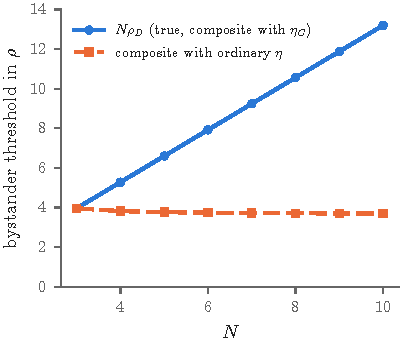
\includegraphics[width=\textwidth]{fig4a_composite_threshold.pdf}
\caption{Bystander threshold}
\end{subfigure}\hfill
\begin{subfigure}[t]{0.47\textwidth}\centering
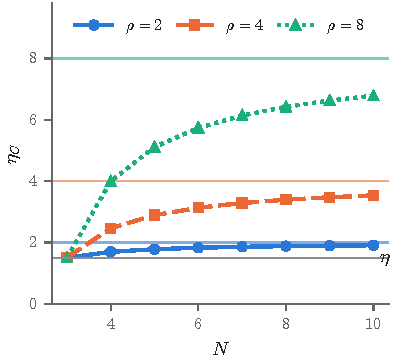
\includegraphics[width=\textwidth]{fig4b_eta_C.pdf}
\caption{Effective elasticity $\eta_C$}
\end{subfigure}
\caption{The composite bystander. (a) The bystander threshold $N\rho_D$, which the composite with $\eta_C$ reproduces, and the threshold of the ordinary-$\eta$ composite, for $N=3,\dots,10$. (b) $\eta_C$ for $\rho\in\{2,4,8\}$, converging toward $\rho$ (thin horizontal lines); the grey line is $\eta=1.5$. \textit{Notes:} illustrative US-like calibration $\alpha_D=0.8$, $\alpha_T=0.4$, $\eta=1.5$.}
\label{fig:composite}
\end{figure}

\begin{proof}[Proof of \cref{prop:real}]
\Cref{eq:realapp,eq:reer} are derived in \cref{app:linear}. For a unilateral tariff $\bar t=d\tau/(N-1)$, so $d\log q_{Ac}/d\tau=(1-\frac{mN}{N-1})\,d\nu_c/d\tau-\frac{m}{N-1}$. Substituting $d\nu_c/d\tau$ from \cref{eq:unilateral} and writing $\frac{m}{N-1}=\frac{mN\,M_N}{N(N-1)M_N}$ gives
\begin{equation*}
\frac{d\log q_{Ac}}{d\tau}=\frac{H_N(\rho)}{N(N-1)M_N(\rho)}.
\end{equation*}
Where MML holds, $M_N>0$, so the response has the sign of $H_N$. Since $\rho_D$ does not depend on $\rho$ and $M_N(\rho)$ in \cref{eq:MN} has slope $dM_N/d\rho=(N-2)/(N-1)$, $H_N$ is affine in $\rho$ with slope
\begin{equation*}
\frac{dH_N}{d\rho}=1-\frac{mN}{N-1}-\frac{mN(N-2)}{N-1}=1-mN.
\end{equation*}

(i) If $m<1/N$, the slope is positive, so $H_N$ has a unique root, is negative below it and positive above it. Multiplying $H_N=0$ by $N-1$ gives $[(N-1)-mN](\rho-N\rho_D)=mN[1+N\alpha_D(\eta-1)+(N-2)\rho]$; the coefficient on $\rho$ is $(N-1)-mN-mN(N-2)=(N-1)(1-mN)$, which yields $\rho^*_q(N)$. At the root $[(N-1)-mN](\rho^*_q-N\rho_D)=mN(N-1)M_N(\rho^*_q)$. For $m<1/N$ the coefficient $(N-1)-mN$ is positive, and if MML holds at $\rho^*_q$ the right-hand side is positive, so $\rho^*_q(N)>N\rho_D$.

(ii) If $m=1/N$, the slope is zero, and
\begin{equation*}
H_N=\frac{N-2}{N-1}(\rho-N\rho_D)-\frac{1+N\alpha_D(\eta-1)+(N-2)\rho}{N-1}=-\frac{1+N\alpha_D(\eta-1)+N(N-2)\rho_D}{N-1}.
\end{equation*}

(iii) If $m>1/N$, the slope is negative.

(iv) If $\eta\geq1$, every term of $M_N$ in \cref{eq:MN} is nonnegative and the first is positive, so MML holds for every $\rho>0$. Since $(N-1)M_N(0)=1+N\alpha_D(\eta-1)$,
\begin{equation*}
(N-1)H_N(0)=-[(N-1)-mN]N\rho_D-mN[1+N\alpha_D(\eta-1)]=-N\big[(N-1)(\rho_D-m)+Nm^2\big],
\end{equation*}
where the second equality uses $\rho_D=1+\alpha_D(\eta-1)-m$. With $\eta\geq1$, $\rho_D-m=1+\alpha_D(\eta-1)-2m\geq1-2m$, so
\begin{align*}
(N-1)(\rho_D-m)+Nm^2&\geq(N-1)(1-2m)+Nm^2=Nm^2-2(N-1)m+(N-1)\\
&=N\Big(m-\frac{N-1}{N}\Big)^2+\frac{N-1}{N}>0.
\end{align*}
Hence $H_N(0)<0$. For $m\geq1/N$, $dH_N/d\rho=1-mN\leq0$, so $H_N(\rho)\leq H_N(0)<0$ and $d\log q_{Ac}/d\tau<0$ for every $\rho>0$.

(v) Under MML $M_N>0$, and $\rho_D>0$. In \cref{eq:reer}, the first term is nonpositive when $m\leq(N-1)/N$ and the second, $-m/(N-1)$, is strictly negative, so the REER strictly appreciates, including at $m=(N-1)/N$. Under weak home bias, $m=\alpha_T(1-\alpha_D)\leq1-1/N=(N-1)/N$.
\end{proof}

\begin{proof}[Proof of \cref{prop:retaliation}]
(i) Let primes denote responses to the mirror shock $t_{BA}=d\tau$. Relabeling $A\leftrightarrow B$ in \cref{eq:unilateral} gives
\begin{equation*}
d\log e'_{BA}=-\frac{N\rho_D+(N-2)\rho}{N(N-1)M_N}\,d\tau,\qquad d\log e'_{Bc}=\frac{\rho-N\rho_D}{N(N-1)M_N}\,d\tau.
\end{equation*}
Since $e_{AB}=1/e_{BA}$ and $e_{Ac}=e_{AB}e_{Bc}$, $d\log e'_{AB}=\frac{N\rho_D+(N-2)\rho}{N(N-1)M_N}d\tau$ and $d\log e'_{Ac}=\frac{\rho}{NM_N}d\tau$. By linearity the combined response is $d\log e_{AB}=0$ and
\begin{equation*}
d\log e_{Ac}=\frac{\rho-N\rho_D}{N(N-1)M_N}\,d\tau+\frac{\rho}{NM_N}\,d\tau=\frac{\rho-\rho_D}{(N-1)M_N}\,d\tau.
\end{equation*}
The three components are $A$'s average protection, $-\rho_D/[(N-1)M_N]$, $A$'s relative treatment, $\rho/[N(N-1)M_N]$, and $B$'s relative treatment, $\rho/(NM_N)$. By symmetry between $A$ and $B$ the same expression applies to $d\log e_{Bc}$, every bystander moves identically, so cross rates among bystanders are unchanged, and averaging over $A$'s $N-1$ partners with the equal weights of the symmetric benchmark gives $d\nu^E_A$ in \cref{eq:retaliation}.

(ii) Superpose the $N$ tariff vectors. $A$'s tariff vector is uniform, $\bar t^{(A)}=d\tau$ and $\widetilde t^{(A)}=0$, and contributes $\lambda_{\mathrm{avg}}d\tau$ to every $d\log e_{Aj}$. Partner $j$ taxes only $A$; its contribution to $d\log e_{Aj}$ is $-[\lambda_{\mathrm{avg}}+(N-2)\lambda_{\mathrm{rel}}]\frac{d\tau}{N-1}$, while each of the $N-2$ other partners $k$ contributes $-\lambda_{\mathrm{rel}}d\tau=\frac{\rho}{NM_N}d\tau$, computed as in part (i) from $e_{Aj}=e_{Ak}e_{kj}$. Summing,
\begin{equation*}
d\log e_{Aj}=\lambda_{\mathrm{avg}}d\tau-\big[\lambda_{\mathrm{avg}}+(N-2)\lambda_{\mathrm{rel}}\big]\frac{d\tau}{N-1}-(N-2)\lambda_{\mathrm{rel}}d\tau=\frac{(N-2)(\rho-\rho_D)}{(N-1)M_N}\,d\tau.
\end{equation*}
The expression is the same for every $j$, so it equals the effective response, and all cross rates among $A$'s partners are unchanged. Under MML the signs are those of $\rho-\rho_D$.
\end{proof}

\begin{proof}[Proof of \cref{lem:welfare}]
Utility is Cobb--Douglas over the tradable aggregate and the non-tradable, so indirect utility is $V_A=\kappa\,I_A/(P_{TA}^{\alpha_T}P_{NA}^{1-\alpha_T})$ for a constant $\kappa$, with $I_A$, $P_{TA}$ and $P_{NA}$ in $A$'s currency. The marginal utility of income is $V_A/I_A$, so the change in welfare in units of income is
\begin{equation*}
\frac{dV_A}{(\partial V_A/\partial I_A)\,I_A}=d\log I_A-\alpha_T\,d\log P_{TA}-(1-\alpha_T)\,d\log P_{NA}.
\end{equation*}
This is the envelope theorem: by Shephard's lemma, $\alpha_T\,d\log P_{TA}=\sum_j s_{Aj}\,d\log p_{Aj}$, the expenditure-share-weighted change in consumer prices. Under the producer-price normalization $w_A=A_{TA}$ and $P_{NA}=A_{TA}/A_{NA}$ are fixed in $A$'s currency, so $d\log P_{NA}=0$ and the domestic tradable's price does not move. Imported goods' consumer prices move by $d\log p_{Aj}=d\nu_j+d\log(1+\tau_{Aj})=d\nu_j+d\tau_{Aj}$ at free trade. Income is labor income plus rebated revenue, $I_A=w_AL_A/(1-\sum_j\theta_{Aj}s_{Aj})$ with $\theta_{Aj}=\tau_{Aj}/(1+\tau_{Aj})$. At free trade $\theta_{Aj}=0$ and $d\theta_{Aj}=d\tau_{Aj}$, so changes in realized shares drop out and $d\log I_A=\sum_js_{Aj}\,d\tau_{Aj}$: the revenue gain equals the tariff change times the border value of imports. Combining,
\begin{equation*}
\frac{dV_A}{(\partial V_A/\partial I_A)\,I_A}=\sum_js_{Aj}\,d\tau_{Aj}-\sum_js_{Aj}(d\nu_j+d\tau_{Aj})=-\sum_js_{Aj}\,d\nu_j=-m_A\sum_{j\neq A}b_{Aj}\,d\nu_j,
\end{equation*}
with $m_A=\sum_js_{Aj}=\alpha_T(1-h_A)$ and $b_{Aj}=s_{Aj}/m_A$. The tariff terms cancel: at free trade the revenue raised exactly offsets the direct price increase to first order. Tariffs imposed by other countries enter $A$'s prices and income only through $d\nu$, so the formula holds for any tariff vector.
\end{proof}

\noindent The replication code checks \cref{lem:welfare} against central finite differences of $A$'s log indirect utility in the nonlinear model, at symmetric and asymmetric free-trade baselines ($N=3,4,5$) and under unilateral, retaliatory, multilateral-war, foreign-only and random tariff shocks; the two agree to within $10^{-6}$.

\begin{proof}[Proof of \cref{prop:uniform}]
Work with the linearized system \cref{eq:linear} at a balanced free-trade baseline, with country-specific $\eta_i$, $\rho_i$ and $\alpha_T^i$, so that $s_{Aj}=\alpha_T^A(1-h_A)b_{Aj}$ and $m_A=\sum_{j\neq A}s_{Aj}=\alpha_T^A(1-h_A)$.

\emph{Step 1: only $A$'s import flows are disturbed.} Set $d\nu=0$ and $d\tau_{Aj}=dt$ for all $j\neq A$, with all other tariff changes zero. For $i\neq A$, $d\tau_{ij}=0$, so $dp_{ij}=0$ for every $j$, $d\log P_{Mi}=0$, $d\log s_{ij}=0$ and $d\log\tilde I_i=0$. Every flow $f_{ij}$ with $i\neq A$ is therefore unchanged. In the trade balance of partner $j$, the only term that moves is its exports to $A$:
\begin{equation*}
F_j=d\TB_j\big|_{d\nu=0}=f_{Aj}\big(d\log s_{Aj}+d\log\tilde I_A-dt\big).
\end{equation*}

\emph{Step 2: the cross-origin margin drops out.} In $A$, $dp_{Aj}=dt$ for every $j$, so $d\log P_{MA}=\sum_jb_{Aj}dt=dt$ and $dp_{Aj}-d\log P_{MA}=0$ for every $j$. The term multiplying $(1-\rho_A)$ vanishes, and
\begin{equation*}
d\log s_{Aj}=(1-\eta_A)h_A\,dt\quad\text{for every }j,\qquad d\log\tilde I_A=\sum_js_{Aj}\,dt=m_A\,dt.
\end{equation*}

\emph{Step 3: the disturbance.} Substituting,
\begin{equation*}
F_j=f_{Aj}\big[(1-\eta_A)h_A+\alpha_T^A(1-h_A)-1\big]dt=-f_{Aj}\big[\eta_Ah_A+(1-h_A)(1-\alpha_T^A)\big]dt=-f_{Aj}\,\rho_D^A\,dt,
\end{equation*}
which is \cref{eq:uniformF}. Since $\eta_A>0$, $0<h_A\leq1$ and $\alpha_T^A\leq1$, $\rho_D^A>0$, so $F_j\leq0$ for every $j$, with $F_j<0$ whenever $f_{Aj}>0$.

\emph{Step 4: exchange rates.} Under MML, $(-J)^{-1}\geq0$, so by \cref{eq:signrule} $d\nu_i=\sum_j\vartheta_{ij}F_j\leq0$ for every $i$: $A$ appreciates weakly against every partner. If $A$ imports from every partner, then $F_j<0$ for all $j$; since $(-J)^{-1}$ is nonsingular and nonnegative, each of its rows has a strictly positive entry, so $d\nu_i<0$ for every $i$. If instead $J$ is irreducible, $-J$ is an irreducible nonsingular M-matrix and $(-J)^{-1}>0$ entrywise, so $d\nu_i<0$ for every $i$ as long as $F\neq0$, that is, as long as $A$ imports at all.

\emph{Step 5: welfare.} By \cref{lem:welfare}, $dU_A/(U_A'I_A)=-m_A\sum_jb_{Aj}d\nu_j\geq0$, and it is strictly positive whenever some $d\nu_j<0$ with $b_{Aj}>0$, which holds in either case of Step 4 because the $b_{Aj}$ sum to one. Since $A$'s aggregate terms of trade improve if and only if $\sum_jb_{Aj}d\nu_j<0$, they improve. Finally, the response is linear in the tariff vector, so the welfare effect of the uniform tariff is $\sum_jg_j\,dt$ with $g_j$ as in \cref{eq:gradient}, and $\sum_jg_j>0$.
\end{proof}

\noindent The replication code checks \cref{eq:uniformF} against the linear system to $10^{-12}$ and against complex-step derivatives of the exact model's trade balances, and verifies the signs of $F$, $d\nu$ and the welfare change on 60 random asymmetric baselines with country-specific parameters ($N=3,4,5$).

\begin{proof}[Proof of \cref{prop:threecases}]
Under MML $\det A(\rho)>0$, so $R_{A|B}$ has the sign of $Q_{A|B}(\rho)$. (a) At the symmetric benchmark, \cref{eq:threecountry} gives $\det A=3(mM_3/2)^2$ and $R_{A|B}=d\nu^E_A/d\tau=-\rho_D/(2M_3)$, so $Q=-\tfrac38m^2\rho_DM_3$, which is affine in $\rho$ ($q_2=0$) and negative for all $\rho$ under MML. (b) If $q_2>0$ and $q_0<0$, the product of the roots is $q_0/q_2<0$, so there is exactly one positive root $\rho^*$, with $Q<0$ on $(0,\rho^*)$ and $Q>0$ beyond. (c) If $q_2<0$, $q_1>0$, $q_0<0$ and the discriminant is positive, both roots are real with positive sum $-q_1/q_2$ and positive product $q_0/q_2$, so both are positive, and the downward parabola is positive only between them.
\end{proof}

\section{Further Results and Data}

This appendix states sufficient conditions for the two-country sign result of \cref{sec:bilateral}, derives the real-exchange-rate results discussed in \cref{sec:composite}, and documents the 2025 data. Throughout, $e_{Aj}$ is units of $A$'s currency per unit of $j$'s currency, so a rise is a depreciation of $A$ against $j$.

\subsection{Two-country sufficient conditions}
\label{app:online-twocountry}

Let $e\equiv e_{AB}$ and let $\tau$ be $A$'s tariff on imports from $B$. Border prices are one in the producer's currency, so with import and export quantities $Q_M$ and $Q_X$, $A$'s import payments are $M_A=eQ_M$, its export receipts are $X_A=Q_X$, and $\TB_A(e,\tau)\equiv X_A(e,\tau)-M_A(e,\tau)$, where $X_A$ and $M_A$ include all induced effects, including income effects of tariff revenue. If $\TB_A$ is continuously differentiable with $\TB_{A,e}\neq0$ at an equilibrium, the implicit function theorem gives a locally unique $e(\tau)$ with $de/d\tau=-\TB_{A,\tau}/\TB_{A,e}$.

The first condition is $\TB_{A,\tau}>0$. Because $M_A=eQ_M$ is measured at border prices, import payments fall at fixed $e$ if and only if the import quantity falls. Under a lump-sum rebate of revenue, with $\varepsilon^H$ the compensated own-price elasticity of import demand, $\eta_I$ its income elasticity and $\theta$ the revenue share of income,
\begin{equation*}
\frac{d\log Q_M}{d\log(1+\tau)}\bigg|_e=-\frac{\varepsilon^H}{1-\eta_I\theta},
\end{equation*}
so at free trade ($\theta=0$) the import quantity falls if and only if $\varepsilon^H>0$. In the nested-CES model at free trade, $\varepsilon^H=\rho_D>0$, the domestic diversion margin of \cref{eq:twocountry}, and $X_{A,\tau}=0$ because $B$'s income and demand are unchanged at a fixed exchange rate. The second condition is $\TB_{A,e}>0$, which at a balanced baseline is equivalent to the Marshall--Lerner condition $\varepsilon_X+\varepsilon_M>1$ (\cref{sec:bilateral}).

When both conditions hold, $de/d\tau<0$. These are sufficient conditions, not properties of every model: the fiscal closure (revenue wasted, spent by the government or transferred abroad) and the pricing convention (local- or dominant-currency pricing, incomplete pass-through, markups) change the quantity responses and can reverse either sign.

\subsection{Real exchange rates}
\label{sec:real}

Let $P_i=P_{Ti}^{\alpha_T}P_{Ni}^{1-\alpha_T}$ be $i$'s consumer price index in its own currency and $q_{Aj}\equiv e_{Aj}P_j/P_A$ the real bilateral exchange rate, so that a rise is a real depreciation of $A$. At the symmetric benchmark the real effective exchange rate is $d\log q^E_A\equiv\frac{1}{N-1}\sum_{j\neq A}d\log q_{Aj}$. With $P_{Ni}$ fixed, $d\log P_i=m\,d\log P_{Mi}$, so $d\log q_{Aj}=d\nu_j+m\,(d\log P_{Mj}-d\log P_{MA})$. Let $A$ impose $t$ and its partners impose none. With equal import weights, $d\log P_{MA}=d\nu^E_A+\bar t$ and $d\log P_{Mj}=d\nu^E_A-\frac{N}{N-1}d\nu_j$, so
\begin{equation}
d\log q_{Aj}=\Big(1-\frac{mN}{N-1}\Big)d\nu_j-m\bar t,
\label{eq:realapp}
\end{equation}
where $-m\bar t$ is the direct effect of the tariff on $A$'s consumer price index. For a unilateral tariff, $\bar t=d\tau/(N-1)$, and averaging with \cref{eq:unilateral},
\begin{equation}
\frac{d\log q^E_A}{d\tau}=-\Big(1-\frac{mN}{N-1}\Big)\frac{\rho_D}{(N-1)M_N}-\frac{m}{N-1}.
\label{eq:reer}
\end{equation}

\begin{proposition}[Real exchange rates]
\label{prop:real}
Consider a marginal unilateral tariff $d\tau>0$ by $A$ on $B$ at the symmetric benchmark, $N\geq3$, $m>0$, partners imposing no tariffs, and define
\begin{equation*}
H_N(\rho)\equiv\Big(1-\frac{mN}{N-1}\Big)(\rho-N\rho_D)-mN\,M_N(\rho).
\end{equation*}
For every untariffed bystander $c$, if $M_N(\rho)\neq0$, $d\log q_{Ac}/d\tau=H_N(\rho)/[N(N-1)M_N(\rho)]$, so wherever MML holds the real bilateral response has the sign of $H_N(\rho)$. Since $\rho_D$ does not depend on $\rho$, $dH_N/d\rho=1-mN$.
\begin{enumerate}[label=(\roman*)]
\item If $m<1/N$, $H_N$ has the unique root
\begin{equation*}
\rho^*_q(N)=\frac{[(N-1)-mN]N\rho_D+mN[N\alpha_D(\eta-1)+1]}{(N-1)(1-mN)}.
\end{equation*}
Where MML holds, $A$ appreciates in real terms against $c$ for $\rho<\rho^*_q(N)$ and depreciates for $\rho>\rho^*_q(N)$; if MML holds at $\rho^*_q(N)$, then $\rho^*_q(N)>N\rho_D$.
\item If $m=1/N$, $H_N$ does not depend on $\rho$: $H_N=-[1+N\alpha_D(\eta-1)+N(N-2)\rho_D]/(N-1)$.
\item If $m>1/N$, $H_N$ is decreasing in $\rho$, so any crossing has the reverse orientation.
\item If $\eta\geq1$, so that MML holds for every $\rho>0$, and $m\geq1/N$, then $H_N(\rho)<0$ for every $\rho>0$: no positive $\rho$ produces a real depreciation against an untariffed bystander.
\item Under MML, if $m\leq(N-1)/N$, $A$'s REER appreciates. Under weak home bias this condition holds automatically, since $m=\alpha_T(1-\alpha_D)\leq(N-1)/N$.
\end{enumerate}
\end{proposition}

At the US-like calibration and $N=3$, $m=0.08<1/3$ and $\rho^*_q=4.93$, against the nominal threshold $3\rho_D=3.96$.

At the US-like calibration and $N=3$, $m=0.08<1/3$ and $\rho^*_q=4.93$, against the nominal threshold $3\rho_D=3.96$.

\begin{proof}[Proof of \cref{prop:real}]
MML is used only for the sign statements in (i), (iii) and (v) and for the comparison in (i); in (iv) it follows from $\eta\geq1$. By \cref{eq:realapp} with $\bar t=d\tau/(N-1)$, $d\log q_{Ac}/d\tau=(1-\frac{mN}{N-1})\,d\nu_c/d\tau-\frac{m}{N-1}$. Substituting $d\nu_c/d\tau$ from \cref{eq:unilateral} and writing $\frac{m}{N-1}=\frac{mN\,M_N}{N(N-1)M_N}$ gives the stated response. Under MML $M_N>0$, so the response has the sign of $H_N$. Since $M_N$ in \cref{eq:MN} has slope $(N-2)/(N-1)$, $H_N$ is affine in $\rho$ with slope $1-\frac{mN}{N-1}-\frac{mN(N-2)}{N-1}=1-mN$.

(i) For $m<1/N$ the slope is positive. Multiplying $H_N=0$ by $N-1$ gives $[(N-1)-mN](\rho-N\rho_D)=mN[1+N\alpha_D(\eta-1)+(N-2)\rho]$; the coefficient on $\rho$ is $(N-1)-mN-mN(N-2)=(N-1)(1-mN)$, which yields $\rho^*_q(N)$. At the root $[(N-1)-mN](\rho^*_q-N\rho_D)=mN(N-1)M_N(\rho^*_q)$. For $m<1/N$ the coefficient $(N-1)-mN$ exceeds $N-2\geq1$, and if MML holds at $\rho^*_q$ the right-hand side is strictly positive because $m>0$ and $M_N(\rho^*_q)>0$; hence $\rho^*_q(N)>N\rho_D$.

(ii) For $m=1/N$ the slope is zero, and $H_N=\frac{N-2}{N-1}(\rho-N\rho_D)-\frac{1+N\alpha_D(\eta-1)+(N-2)\rho}{N-1}$, which reduces to the stated constant.

(iii) For $m>1/N$ the slope is negative.

(iv) If $\eta\geq1$, every term of $M_N$ in \cref{eq:MN} is nonnegative and the first is positive, so MML holds for every $\rho>0$. Since $(N-1)M_N(0)=1+N\alpha_D(\eta-1)$ and $\rho_D=1+\alpha_D(\eta-1)-m$,
\begin{equation*}
(N-1)H_N(0)=-[(N-1)-mN]N\rho_D-mN[1+N\alpha_D(\eta-1)]=-N\big[(N-1)(\rho_D-m)+Nm^2\big].
\end{equation*}
With $\eta\geq1$, $\rho_D-m\geq1-2m$, so
\begin{equation*}
(N-1)(\rho_D-m)+Nm^2\geq Nm^2-2(N-1)m+(N-1)=N\Big(m-\frac{N-1}{N}\Big)^2+\frac{N-1}{N}>0.
\end{equation*}
Hence $H_N(0)<0$. For $m\geq1/N$, $dH_N/d\rho\leq0$, so $H_N(\rho)\leq H_N(0)<0$ for every $\rho>0$.

(v) Under MML $M_N>0$, and $\rho_D>0$. In \cref{eq:reer}, the first term is nonpositive if and only if $m\leq(N-1)/N$, and the second, $-m/(N-1)$, is strictly negative because $m>0$. Under weak home bias, $1-\alpha_D\leq(N-1)/N$ and $\alpha_T\leq1$, so $m=\alpha_T(1-\alpha_D)\leq(N-1)/N$.
\end{proof}

\subsection{Data notes for the 2025 episode}
\label{app:episode-data}

\paragraph{Exchange-rate data.} Bilateral rates are Federal Reserve H.10 noon buying rates, expressed in dollars per unit of foreign currency (the CNY, CAD and MXN quotes are inverted). The broad index is the H.10 nominal broad dollar index (goods and services), which rises when the dollar appreciates; it is inverted. The index excluding China removes the renminbi from the daily log change of the broad index using China's 2025 H.10 weight (10.9 percent) and divides by one minus that weight, so the remaining weights are renormalized to sum to one. No daily dong series is available from the H.10 release or from the BIS; the VND row of \cref{tab:phases} uses BIS monthly averages in the monthly columns and, in the daily columns (marked $^{a}$), BIS end-of-month rates for the same months (end-January to end-March, end-March to end-April, end-July to end-December). Sources: FRED (DEXUSEU, DEXCHUS, DEXCAUS, DEXMXUS, DTWEXBGS), Federal Reserve H.10 trade weights and BIS (VND). ``Monthly'' compares monthly averages, January with March (Phase~1), March with April (Phase~2) and July with December (Phase~3), windows that do not coincide with the phase dates; ``daily'' runs from January~31 to April~2, April~2 to May~12 and August~6 to December~31. Panel~(a) of \cref{fig:episode} plots monthly averages, at mid-month, relative to each series' January~2025 average; the August dong average is missing in the source.

\paragraph{Tariff data.} Panel~(b) of \cref{fig:episode} plots statutory headline tariffs above the pre-2025 baseline by effective date: US tariffs on China, which reached 145 percent on April~10 and were reduced to 30 percent on May~14; China's across-the-board tariffs on the United States, which reached 125 percent on April~12; US tariffs on the European Union; the 10 percent US baseline on unlisted partners from April~5; US tariffs on Canada; and Canada's tariffs on covered US goods. Section~232 product tariffs, exclusions and de minimis changes are omitted, and rates are not trade-weighted. US measures are from Federal Register executive orders and Canadian measures from the Department of Finance Canada; Chinese measures are as reported in USDA Foreign Agricultural Service summaries of State Council Tariff Commission announcements. The complete chronology of effective dates and rates is in the online supplement.

\paragraph{Phase definitions.} Phase~1 (February~1--April~2) covers the two US tariff increases on China and China's product-specific responses. Phase~2 (April~3--May~12) covers the US--China escalation, the 10 percent baseline of April~5, from which Canada and Mexico were excluded, and the higher country-specific rates of April~9, which were suspended for every partner except China on April~10. Phase~3 (August~7--December~31) begins with the August framework rates.

\paragraph{Classification caveats.} The phase classifications are approximate. Tariffs on Canada and Mexico, partial retaliation, exclusions, and contemporaneous policy announcements mean that none of the phases is a clean experiment. Vietnam also shifted between bystander-like and targeted treatment during the year. The online supplement documents these complications and the complete tariff chronology.

The online supplement also considers sector-specific factors and permanent trade imbalances. These extensions shift quantitative thresholds without changing the central mechanism.

\subsection{Illustrative U.S.--China--rest-of-world mapping}
\label{app:usmap}

This mapping places a unilateral US tariff on China in the three-country model, with $A$ the United States, $B$ China and $C$ the rest of the world. It maps trade shares and country sizes; it is not a calibration of exchange-rate magnitudes.

All inputs are for 2024, in billions of current dollars. US goods imports are $3{,}266.4$ in total and $440.3$ from China, and US goods exports $2{,}061.7$ in total and $143.3$ to China (US Census Bureau). China's goods imports are $2{,}585.1$ in total and $163.6$ from the United States, and its exports $3{,}577.2$ in total and $524.7$ to the United States (China's General Administration of Customs). This gives $b_{AB}=0.135$ and $b_{BA}=0.063$. The rest of the world's imports from the United States are US exports less US exports to China, and its imports from China are China's exports less China's exports to the United States, which gives $b_{CA}=0.386$ and $b_{CB}=0.614$. Country sizes are GDP at purchasing-power parity (IMF World Economic Outlook, October 2026), with the rest of the world equal to world GDP less that of the United States and China; relative to the United States they are $(1,1.30,4.45)$. The origin weights $\beta_{ij}$ are chosen so that the balanced free-trade baseline, solved at $\bar\rho=3\rho_D=3.96$ and then held fixed as $\rho$ varies, reproduces these six shares exactly. The remaining parameters are $\alpha_T=0.4$ and $\eta=1.5$, with either a common $\alpha_D=0.8$ or, for the United States, $\alpha_D=0.673$, the domestic share of US goods absorption in 2024 (BEA goods output plus imports less exports).

The bilateral bystander threshold, above which the dollar depreciates against the rest of the world, is $4.01$ with the common home bias and $3.87$ with the measured US home share. The aggregate terms-of-trade condition \cref{eq:totcondition} fails only for $\rho$ above $4.66$ and $4.50$, respectively. MML holds at both baselines for all $\rho\in[1,20]$. The mapping imposes balanced trade on every country, whereas the observed US goods deficit in 2024 was about $1{,}205$; it ignores the gaps between mirror trade statistics, uses model-implied rather than measured home shares for China and the rest of the world, covers goods only and treats the rest of the world as a single country.

\subsection{Data notes for the 2025 episode}
\label{app:episode-data}

\paragraph{Exchange-rate data.} Bilateral rates are Federal Reserve H.10 noon buying rates, expressed in dollars per unit of foreign currency (the CNY, CAD and MXN quotes are inverted). The broad index is the H.10 nominal broad dollar index (goods and services), which rises when the dollar appreciates; it is inverted. The index excluding China removes the renminbi from the daily log change of the broad index using China's 2025 H.10 weight (10.9 percent) and divides by one minus that weight, so the remaining weights are renormalized to sum to one. No daily dong series is available from the H.10 release or from the BIS; the VND row of \cref{tab:phases} uses BIS monthly averages in the monthly columns and, in the daily columns (marked $^{a}$), BIS end-of-month rates for the same months (end-January to end-March, end-March to end-April, end-July to end-December). Sources: FRED (DEXUSEU, DEXCHUS, DEXCAUS, DEXMXUS, DTWEXBGS), Federal Reserve H.10 trade weights and BIS (VND). ``Monthly'' compares monthly averages, January with March (Phase~1), March with April (Phase~2) and July with December (Phase~3), windows that do not coincide with the phase dates; ``daily'' runs from January~31 to April~2, April~2 to May~12 and August~6 to December~31. Panel~(a) of \cref{fig:episode} plots monthly averages, at mid-month, relative to each series' January~2025 average; the August dong average is missing in the source.

\paragraph{Tariff data.} Panel~(b) of \cref{fig:episode} plots statutory headline tariffs above the pre-2025 baseline by effective date; Section~232 product tariffs, exclusions and de minimis changes are omitted, and rates are not trade-weighted. Effective dates (2025), in percent: US on China 10 (February~4), 20 (March~4), 30 (April~5), 104 (April~9), 145 (April~10), 30 (May~14), 20 (November~10); China on US, across the board, 84 (April~10), 125 (April~12), 10 (May~14), with the product-specific measures of February~10 and March~10 not shown; US on EU 10 (April~5), 20 (April~9 only), 10 (April~10), 15 inclusive of MFN duties (August~7); US baseline on unlisted partners 10 (April~5); US on Canada 25 (March~4), non-USMCA goods only from March~7, 35 (August~1), with the rate on Mexico at 25 from March~4 to year-end (not shown); Canada on US 25 on covered goods (March~4), with coverage widened on March~13 and April~9 and narrowed to steel, aluminium and autos on September~1. US measures are from Federal Register executive orders and Canadian measures from the Department of Finance Canada; Chinese measures are as reported in USDA Foreign Agricultural Service summaries of State Council Tariff Commission announcements.

\paragraph{Phase definitions.} Phase~1 (February~1--April~2) covers the two US tariff increases on China and China's product-specific tariffs of 10--15 percent, on coal, liquefied natural gas, crude oil and some machinery and vehicles from February~10 and on agricultural products from March~10. In Phase~2 (April~3--May~12) the 10 percent baseline took effect on April~5, with Canada and Mexico excluded, and higher country-specific rates took effect on April~9 and were suspended for every partner except China on April~10. Phase~3 (August~7--December~31) begins with the August framework rates. Between the May~12 and August~6 daily observations, which fall outside the phases, the dollar fell by a further $4.9$ percent against the euro and $2.5$ percent against the broad index; in December it was $13.1$ percent weaker against the euro than in January.

\paragraph{Classification caveats.} The US tariffs on Canada (10 percent on energy) and Mexico took effect on March~4 and from March~7 no longer applied to goods qualifying under the USMCA. Canada retaliated on March~4 with a 25 percent surtax on C\$30 billion of US goods \citep{canadafinance2025} and extended it to a further C\$29.8 billion on March~13; Mexico did not retaliate. Canada and Mexico together carry 27.6 percent of the broad index. In the week of March~3--7 the broad index fell by $1.8$ percent, more than its net change over Phase~1, and the dollar fell by $4.4$ percent against the euro. The same week also contained the March~4 announcement by Germany's prospective governing parties of a large defence and infrastructure package and a loosening of the debt brake \citep{ripper2025}. The dollar strengthened against the dong by $3.2$ percent between the January and December averages, all of it by July. Vietnam, however, moved during the year from a bystander-like position to a direct target: a 46 percent rate was announced on April~2 and was in force for one day before the suspension of April~10, and a 20 percent rate applied from August~7. From August~7 to November~10, Vietnam's 20 percent against China's 30 percent was relative treatment in Vietnam's favour; after November~10, when both faced 20 percent, it disappeared. Within Phase~3 the dollar was roughly flat against the dong ($0.0$ percent on monthly averages, $+0.5$ percent between end-of-month rates).

\section{Further Robustness}
\label{app:online}

This appendix states sufficient conditions for the two-country sign result of \cref{sec:bilateral}. Throughout, $e_{Aj}$ is units of $A$'s currency per unit of $j$'s currency, so a rise is a depreciation of $A$ against $j$.

\subsection{Two-country sufficient conditions}
\label{app:online-twocountry}

Let $e\equiv e_{AB}$ and let $\tau$ be $A$'s tariff on imports from $B$. Border prices are one in the producer's currency, so with import and export quantities $Q_M$ and $Q_X$, $A$'s import payments are $M_A=eQ_M$, its export receipts are $X_A=Q_X$, and $\TB_A(e,\tau)\equiv X_A(e,\tau)-M_A(e,\tau)$, where $X_A$ and $M_A$ include all induced effects, including income effects of tariff revenue. If $\TB_A$ is continuously differentiable with $\TB_{A,e}\neq0$ at an equilibrium, the implicit function theorem gives a locally unique $e(\tau)$ with $de/d\tau=-\TB_{A,\tau}/\TB_{A,e}$.

The first condition is $\TB_{A,\tau}>0$. Because $M_A=eQ_M$ is measured at border prices, import payments fall at fixed $e$ if and only if the import quantity falls. Under a lump-sum rebate of revenue, with $\varepsilon^H$ the compensated own-price elasticity of import demand, $\eta_I$ its income elasticity and $\theta$ the revenue share of income,
\begin{equation*}
\frac{d\log Q_M}{d\log(1+\tau)}\bigg|_e=-\frac{\varepsilon^H}{1-\eta_I\theta},
\end{equation*}
so at free trade ($\theta=0$) the import quantity falls if and only if $\varepsilon^H>0$. In the nested-CES model at free trade, $\varepsilon^H=\rho_D>0$, the domestic diversion margin of \cref{eq:twocountry}, and $X_{A,\tau}=0$ because $B$'s income and demand are unchanged at a fixed exchange rate. The second condition is $\TB_{A,e}>0$, which at a balanced baseline is equivalent to the Marshall--Lerner condition $\varepsilon_X+\varepsilon_M>1$ (\cref{sec:bilateral}).

When both conditions hold, $de/d\tau<0$. These are sufficient conditions, not properties of every model: the fiscal closure (revenue wasted, spent by the government or transferred abroad) and the pricing convention (local- or dominant-currency pricing, incomplete pass-through, markups) change the quantity responses and can reverse either sign.

The online supplement also considers sector-specific factors and permanent trade imbalances. These extensions preserve the qualitative mechanism while shifting the quantitative bystander threshold.


\end{document}
